\documentclass[11pt,a4paper]{article}

% ─── Packages ────────────────────────────────────────────────────────────────
\usepackage[utf8]{inputenc}
\usepackage[T1]{fontenc}
\usepackage{lmodern}
\usepackage{geometry}
\usepackage{amsmath,amssymb,amsthm}
\usepackage{hyperref}
\usepackage{listings}
\usepackage{xcolor}
\usepackage{booktabs}
\usepackage{graphicx}
\usepackage{fancyhdr}
\usepackage{tikz}
\usetikzlibrary{arrows.meta,positioning,fit,backgrounds,calc,shapes.geometric,shapes.symbols,decorations.pathmorphing,decorations.pathreplacing}
\usepackage{float}
\usepackage{caption}
\usepackage{enumitem}

% ─── Geometry ────────────────────────────────────────────────────────────────
\geometry{margin=2.5cm}

% ─── Colors ──────────────────────────────────────────────────────────────────
\definecolor{codebg}{RGB}{248,248,248}
\definecolor{codeframe}{RGB}{200,200,200}
\definecolor{darkgreen}{HTML}{00564C}
\definecolor{darkblue}{HTML}{003FB8}
\definecolor{accent}{HTML}{00564C}
\definecolor{hhsand}{HTML}{E9DCC4}
\definecolor{hhsanddeep}{HTML}{D8C7A6}
\definecolor{hhebony}{HTML}{121212}
\definecolor{hhink}{HTML}{1B1712}
\definecolor{hhcobalt}{HTML}{003FB8}
\definecolor{hhamber}{HTML}{6B4500}
\definecolor{hhteal}{HTML}{00564C}
\definecolor{hhpaper}{HTML}{FBF7EF}

% Verification-status markers, matching the Anchor / Bonded conventions.
\newcommand{\Closed}{{\textcolor{hhteal}{\textbf{\textsf{closed}}}}}
\newcommand{\Partial}{{\textcolor{hhamber}{\textbf{\textsf{partial}}}}}
\newcommand{\Open}{{\textcolor{hhcobalt}{\textbf{\textsf{open}}}}}

% Pull-quote sidebar: large quote, left-edge accent stripe.
\newcommand{\pullquote}[1]{%
  \par\vspace{6pt}%
  \noindent\begin{tikzpicture}
    \node[draw=none,fill=hhsand!40,line width=0pt,
          inner sep=10pt,text width=\dimexpr\textwidth-30pt\relax,
          align=left] (q) {%
      \sffamily\itshape\large #1%
    };
    \draw[hhcobalt,line width=2.5pt] (q.north west) -- (q.south west);
  \end{tikzpicture}\par\vspace{6pt}%
}

% ─── Listings Setup ──────────────────────────────────────────────────────────
\lstdefinestyle{proverif}{
  language=C,
  backgroundcolor=\color{codebg},
  frame=single,
  rulecolor=\color{codeframe},
  basicstyle=\ttfamily\small,
  keywordstyle=\color{darkblue}\bfseries,
  commentstyle=\color{darkgreen}\itshape,
  stringstyle=\color{accent},
  numbers=left,
  numberstyle=\tiny\color{gray},
  numbersep=8pt,
  breaklines=true,
  showstringspaces=false,
  tabsize=2,
  xleftmargin=15pt,
  xrightmargin=5pt,
  framexleftmargin=15pt,
  captionpos=b
}
\lstdefinestyle{tlaplus}{
  backgroundcolor=\color{codebg},
  frame=single,
  rulecolor=\color{codeframe},
  basicstyle=\ttfamily\small,
  keywordstyle=\color{darkblue}\bfseries,
  commentstyle=\color{darkgreen}\itshape,
  stringstyle=\color{accent},
  numbers=left,
  numberstyle=\tiny\color{gray},
  numbersep=8pt,
  breaklines=true,
  showstringspaces=false,
  tabsize=2,
  xleftmargin=15pt,
  xrightmargin=5pt,
  framexleftmargin=15pt,
  captionpos=b,
  morekeywords={MODULE,EXTENDS,CONSTANTS,VARIABLES,VARIABLE,Init,Next,Spec,
    TypeOK,IF,THEN,ELSE,LET,IN,CHOOSE,SUBSET,UNION,DOMAIN,EXCEPT,
    UNCHANGED,TRUE,FALSE,BOOLEAN,Nat,Int,STRING,Seq,Append,Len,Head,Tail,
    ENABLED,WF_,SF_,THEOREM,ASSUME,INSTANCE,WITH,LOCAL}
}
\lstset{style=proverif}

% ─── Theorem Environments ────────────────────────────────────────────────────
\theoremstyle{definition}
\newtheorem{definition}{Definition}[section]
\newtheorem{theorem}{Theorem}[section]
\newtheorem{lemma}{Lemma}[section]
\newtheorem{property}{Property}[section]
\newtheorem{corollary}{Corollary}[section]

\theoremstyle{remark}
\newtheorem*{remark}{Remark}

% ─── Header/Footer ───────────────────────────────────────────────────────────
\pagestyle{fancy}
\fancyhf{}
\fancyhead[L]{\small\textit{The Federated Harbor}}
\fancyhead[R]{\small\thepage}
\fancyfoot[C]{\small Port Daddy v4 --- pre-print}
\renewcommand{\headrulewidth}{0.4pt}
\renewcommand{\footrulewidth}{0pt}

% ─── Title ───────────────────────────────────────────────────────────────────
\title{
  \vspace{-1cm}
  {\Large\textsc{Technical White Paper}}\\[0.5cm]
  \rule{\textwidth}{0.5pt}\\[0.3cm]
  {\LARGE\textbf{The Federated Harbor:}}\\[0.2cm]
  {\Large Identity, Coordination, and Settlement\\Across Administrative Domains}\\[0.3cm]
  \rule{\textwidth}{0.5pt}
}
\author{
  \textbf{Erich Owens}\\[0.2cm]
  Curiositech LLC\\[0.2cm]
  \texttt{engineering@portdaddy.dev}
}
\date{May 2026\\Version 0.9 (pre-print)}

% ─── Document ────────────────────────────────────────────────────────────────
\begin{document}

\maketitle
\thispagestyle{empty}

\vspace{1cm}

\begin{abstract}\noindent
A demonstration is scheduled for 4pm. Alice runs the back end on her laptop; Bob runs the front end on his. Each operator has a working local harbor in the sense of the two prior papers in this series --- capability tokens are pinned and attenuated, evidence is Merkle-chained, bonds are posted, and the Conservation invariant holds inside each machine. The problem is not internal. Alice's \texttt{db:write} card is gibberish to Bob's daemon, Bob's revocation gossip is invisible to Alice's mesh, and a bond Alice posted to cover a botched migration sits in her harbor's collateral pool while the migration lands in Bob's staging database. Two harbors, each individually trustworthy, jointly useless. This paper extends the Anchor Protocol's capability ceremony, the Bonded Commons' evidence trail and competitive-insurance market, and the daemon-as-correlation-device argument to settings where the sovereign is not single. We define an inter-harbor capability transfer protocol with explicit attenuation across the boundary; a federated revocation gossip layer with a named convergence bound and cross-witness equivocation detection; a settlement protocol in which a bond posted at one harbor clears against damage measured at another through a structurally bounded escrow; and an admission ceremony for new harbors to join an existing mesh without prior reputation. We are disciplined about which claims are mechanized, which are bounded against named threat windows, and which are honestly open. The point of the paper is to draw the new boundary cleanly so that the unsolved problems are visible rather than hidden.
\end{abstract}

\vspace{0.5cm}
\noindent\textbf{Keywords:} federated identity, capability delegation, cross-realm authorization, mechanism design, distributed trust, certificate transparency, atomic settlement, mutual suspicion.

\vspace{0.4cm}
\noindent\textit{Reading time: approximately 45 minutes end-to-end. The companion papers, \emph{The Anchor Protocol} (Owens 2026) and \emph{The Bonded Commons} (Owens 2026), supply the cryptographic and economic primitives this paper extends. Either of those can be read first or in parallel; this paper is the federation half. The Reader's Map below provides shorter routes for specific audiences.}

\vspace{0.6cm}

% ─── Series locator box (identical template across all three papers) ──────────
\begin{center}
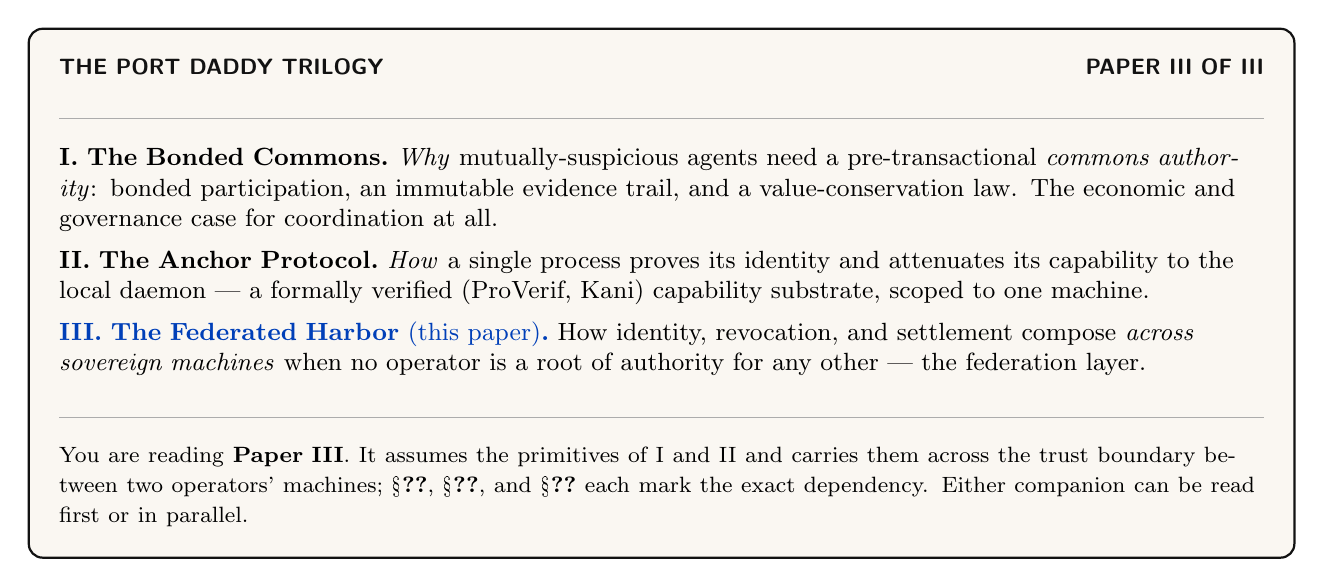
\begin{tikzpicture}
\node[draw=hhebony,line width=0.8pt,rounded corners=5pt,fill=hhsand!22,
      inner sep=11pt,text width=15.3cm,align=left,font=\small] {%
  {\sffamily\bfseries\footnotesize\textcolor{hhebony}{THE PORT DADDY TRILOGY\hfill PAPER~III~OF~III}}\\[5pt]
  {\color{hhebony!35}\rule{\linewidth}{0.4pt}}\\[6pt]
  \textbf{I.~The Bonded Commons.}~\emph{Why} mutually-suspicious agents need a pre-transactional \emph{commons authority}: bonded participation, an immutable evidence trail, and a value-conservation law. The economic and governance case for coordination at all.\\[4pt]
  \textbf{II.~The Anchor Protocol.}~\emph{How} a single process proves its identity and attenuates its capability to the local daemon --- a formally verified (ProVerif, Kani) capability substrate, scoped to one machine.\\[4pt]
  {\color{hhcobalt}\textbf{III.~The Federated Harbor \textnormal{(this paper)}.}}~How identity, revocation, and settlement compose \emph{across sovereign machines} when no operator is a root of authority for any other --- the federation layer.\\[6pt]
  {\color{hhebony!35}\rule{\linewidth}{0.4pt}}\\[5pt]
  {\footnotesize You are reading \textbf{Paper III}. It assumes the primitives of I and II and carries them across the trust boundary between two operators' machines; \S\ref{sec:fh-xfer}, \S\ref{sec:fh-revocation}, and \S\ref{sec:fh-settlement} each mark the exact dependency. Either companion can be read first or in parallel.}
};
\end{tikzpicture}
\end{center}

\vspace{0.4cm}

% ═══════════════════════════════════════════════════════════════════════════════
\section*{Reader's Map}\label{sec:fh-readers-map}
% ═══════════════════════════════════════════════════════════════════════════════

The paper has a topology: it opens with the gestalt (\S\ref{sec:fh-intro}--\S\ref{sec:fh-authority}), then moves through three load-bearing primitives in order of cryptographic depth (capability transfer, revocation, settlement), then steps back to admission, failure modes, and limitations. The figures are designed to be readable in sequence without the surrounding prose; if you want the five-figure summary, that path is given below.

\vspace{0.4cm}
\noindent
\begin{tabular}{p{3.6cm} p{8.6cm} p{3.4cm}}
\toprule
\textbf{Layer} & \textbf{Load-bearing artifact} & \textbf{Lives at} \\
\midrule
\textbf{(1) Topology}        & Two harbors, witness log, settlement escrow as a four-element gestalt & \S\ref{sec:fh-authority}; Figure~\ref{fig:fh-topology} \\
\textbf{(2) Cap.\ transfer}  & Four-message ceremony; ProVerif model of cross-realm authenticity \& attenuation, \emph{conditional on a witness-log freshness assumption} (\S\ref{sec:fh-xfer-mech}) & \S\ref{sec:fh-xfer}; Figure~\ref{fig:fh-xfer} \\
\textbf{(3) Revocation}      & Federated cuckoo-filter mesh; $\Delta(1+\ln m)$ convergence bound & \S\ref{sec:fh-revocation}; Figure~\ref{fig:fh-revocation} \\
\textbf{(4) Settlement}      & Bounded escrow with two-outcome decision space; cross-harbor Conservation & \S\ref{sec:fh-settlement}; Figure~\ref{fig:fh-settlement} \\
\textbf{(5) Threat bands}    & What is mechanized, what is bounded, what is open & \S\ref{sec:fh-limitations}; Figure~\ref{fig:fh-threat-bands} \\
\bottomrule
\end{tabular}

\vspace{0.6cm}
\noindent\textbf{Suggested reading paths by reader type:}
\begin{itemize}[nosep,leftmargin=*,topsep=2pt]
\item \textbf{Beginner / new to the series.} Read \S\ref{sec:fh-intro} (the two-machine problem) and \S\ref{sec:fh-worked-example} (Alice and Bob, end-to-end). The worked example is written to be read cold. Look at the five figures in order. Skip the proofs on the first pass.
\item \textbf{Distributed-systems engineer.} \S\ref{sec:fh-authority} (the topology), \S\ref{sec:fh-xfer} (transfer ceremony), \S\ref{sec:fh-revocation} (gossip and equivocation). The companion Anchor paper for the cryptographic substrate. Then \S\ref{sec:fh-limitations} for the honest open questions.
\item \textbf{Formal-methods reviewer.} Jump to \S\ref{sec:fh-formal} (the TLA+ and ProVerif extensions) and Appendix~\ref{app:fh-mech} (the verification status table). Threat bands in Figure~\ref{fig:fh-threat-bands} are the most concentrated signal of what is and is not mechanized.
\item \textbf{Cryptoeconomic / mechanism-design reader.} \S\ref{sec:fh-settlement} (bounded escrow) and \S\ref{sec:fh-admission} (cold-start admission via bonded sponsorship). The proposal's equilibrium contributions are stated here as open work; that is honest, not coy.
\item \textbf{Security-engineering reviewer.} \S\ref{sec:fh-threat-model} (threat model) first, then the three primitive sections in order. \S\ref{sec:fh-failure-modes} for the operationally interesting cases the protocols do not close.
\end{itemize}

\vspace{0.5cm}
\noindent\textbf{Companion papers.} The Anchor Protocol pins down what it means for a process on a single machine to prove its identity to the local daemon. The Bonded Commons explains why coordination at scale needs a pre-transactional commons authority rather than per-transaction trust negotiation. This paper extends both into the cross-machine, cross-organization case. We will cite specific sections (e.g.\ \emph{Anchor~\S2.4}, \emph{Bonded~\S2}) when we depend on a primitive rather than re-derive it.

\newpage
\tableofcontents
\newpage

% ═════════════════════════════════════════════════════════════════════════════
\section{Introduction: The Two-Machine Problem}\label{sec:fh-intro}
% ═════════════════════════════════════════════════════════════════════════════

A demonstration is scheduled for 4pm. Alice runs the back end of the demo on her laptop; Bob runs the front end on his. Each has a working Port Daddy daemon: capability tokens are minted and attenuated under the Anchor Protocol~\cite{owens2026anchor}, the workspace history is Merkle-chained and replicated locally per the Bonded Commons~\cite{owens2026bonded}, and bonds for cleanup of botched migrations are posted in the local collateral pool. Inside each laptop, the trust story is closed and the formal-verification artifacts hold.

The demo nevertheless does not work. Three failures, none of them inside either machine:

\begin{enumerate}
\item Alice's agent obtains a \texttt{db:write} card for the staging database, attempts to use it against Bob's daemon, and is refused. Bob's daemon has never seen Alice's signing key. The card is well-formed under the Anchor Protocol, but Bob has no root of authority for it; from his daemon's point of view, the card is gibberish.
\item Five minutes before the demo, Alice's operator revokes the \texttt{db:write} card after spotting that it has been over-attenuated. The revocation propagates within Alice's mesh in under a second by the gossip protocol of Anchor~\S4. Bob's harbor never hears about it. The card remains live on Bob's side.
\item The migration runs anyway, lands in Bob's staging database, and corrupts the demo schema. Alice posted a bond in her harbor against exactly this case. The bond sits in her harbor's collateral pool. Bob's harbor measured the damage. Neither harbor can, on its own, route the bond to where the damage is.
\end{enumerate}

Each failure is a different facet of the same underlying gap. Both daemons are internally consistent. Neither is a root of authority for the other. The single-machine sovereign of the prior papers does not extend to the case of two machines under two operators with no shared administrative parent.

We call this the \textbf{two-machine problem}. The point of stating it this baldly is that the failure modes are not exotic; they are what every developer who has tried to dovetail two local agent fleets on a shared task has seen. The bug is structural. The bug is not in either daemon. The bug is in the assumption that one daemon's authority extends past the machine boundary by default. It does not, and it should not.

\pullquote{The trick is not to extend a single sovereign across machines. The trick is to admit there are two and to specify what they owe each other.}

This paper extends the Anchor Protocol, the Bonded Commons, and the daemon-as-correlation-device argument to the multi-administrative-domain case. We are not introducing a new substrate; we are showing that the existing substrate admits a clean federation, and that the federation rules are sharper than they look. Where the prior papers spoke of \emph{the} commons authority, this paper speaks of a \emph{mesh of} mutually witnessing commons authorities, each sovereign inside its own machine, none sovereign over the others, and all of them bound to the same audit substrate.

\subsection{What this paper is and is not}\label{sec:fh-scope}

This paper is the third in a tightly-coupled series. The Anchor Protocol is the cryptographic-token substrate; the Bonded Commons is the economic and governance argument; this paper is the federation layer. The relationships are concrete: \S\ref{sec:fh-xfer} extends Anchor's Phase-3 delegation chain across a trust boundary; \S\ref{sec:fh-revocation} extends Anchor's cuckoo-filter mesh; \S\ref{sec:fh-settlement} extends Bonded's Conservation invariant.

What this paper is \emph{not}: it is not a permissionless-blockchain redesign. Port Daddy daemons do not run consensus. The Federated Harbor explicitly rejects the assumption common to most modern federation proposals~\cite{tobin2017inevitable, schindler2019ethdkg} that a shared ledger is the right substrate. The cost of that simplification is that we cannot lean on a chain for ordering, equivocation detection, or settlement; we must construct each of those primitives from peer gossip plus a federated witness log. The advantage is that the design composes cleanly with the local-first, single-operator-machine architecture of the prior two papers.

\subsection{Contributions}\label{sec:fh-contributions}

The contributions are concrete. We separate them by mechanization status to be honest about which are theorems, which are bounded threat models, and which are sketches.

\begin{enumerate}
\item \textbf{The four-element federation topology (\S\ref{sec:fh-authority}).} A precise statement of the boundary between intra-harbor and inter-harbor scope. Defines harbor sovereignty as a property characterization in the style of Bonded's Admissible KMS, so that subsequent claims can be checked against it.

\item \textbf{The inter-harbor capability transfer ceremony (\S\ref{sec:fh-xfer}).} A four-message protocol exchanging a Harbor Card issued by $A$ for an attenuated card valid at $B$, without either daemon trusting the other's signing key as a root. The ceremony binds the issuing harbor's current epoch root into the envelope, which is the substrate that revocation in \S\ref{sec:fh-revocation} hooks into. ProVerif model in Appendix~\ref{app:fh-proverif} (status: \Partial, model drafted; soundness pending mechanization).

\item \textbf{Federated revocation mesh (\S\ref{sec:fh-revocation}).} The multi-administrative-domain extension of Anchor's cuckoo-filter gossip protocol. Each harbor publishes an epoch root to a shared witness log; cross-witness signatures generalize the Certificate Transparency auditor pattern~\cite{laurie2013ct} to capability tokens. We prove a $\Delta(1+\ln m)$ convergence bound on revocation propagation for $m$ federated harbors gossiping every $\Delta$, and an $O(\log m)$ expected detection bound on cross-witness equivocation (Theorem~\ref{thm:fh-conv}).

\item \textbf{Cross-harbor settlement (\S\ref{sec:fh-settlement}).} A protocol for atomic clearing of a bond posted at $A$ against damage measured at $B$, with a third-party escrow whose role is structurally bounded: it can refuse to clear, but it cannot redirect funds, equivocate about clearing decisions, or extract more than a pre-agreed fee. The bounded-escrow design is inspired by HTLC-style atomic-swap constructions~\cite{herlihy2018atomic} but specialized to a setting where the assets are reputation-priced under competitive insurance, not fungible coins.

\item \textbf{Cold-start admission ceremony (\S\ref{sec:fh-admission}).} A protocol for a new harbor joining an existing mesh without prior reputation, using a bonded-sponsor pattern: an existing harbor posts a bond on the newcomer's behalf, which is forfeit on misbehavior in a probationary epoch. This is the federation-layer analogue of competitive insurance from Bonded.

\item \textbf{Honest open problems (\S\ref{sec:fh-limitations}).} Three named open questions: (a) whether the correlated-equilibrium reframing of Bonded survives the multi-principal setting cleanly; (b) whether bonds can settle without a trusted-but-bounded escrow third party; (c) whether the folk-theorem cartel-resistance argument from Bonded weakens at the federation layer, and by how much. We state these as open, not as solved.
\end{enumerate}

The proposal that scoped this paper~\cite{owens2026proposal} listed two further contributions (a formal definition of harbor sovereignty, and equilibrium results across federations co-authored with Youle) which are present here in skeletal form and will be load-bearing in a subsequent revision once the open problems above resolve. We will not claim a result we do not have.

% ═════════════════════════════════════════════════════════════════════════════
\section{The Federated Authority}\label{sec:fh-authority}
% ═════════════════════════════════════════════════════════════════════════════

The Bonded Commons paper defined a \emph{commons authority} as a pre-transactional trust infrastructure with sovereign scope inside a single machine. Inside that scope, the daemon is the unique correlation device that turns mutually-suspicious agents into a correlated equilibrium~\cite{owens2026bonded}. The single-machine sovereign was an honest simplification. We now drop it.

The federation we build has four elements (Figure~\ref{fig:fh-topology}). Two harbors, each sovereign inside its own machine. A shared witness log to which each harbor publishes its current epoch root, and which any third party can audit for equivocation. A settlement escrow with a structurally bounded decision space. Every primitive in the rest of the paper attaches to one of these four elements.

% Federation topology — the basic gestalt: two harbors, neither root for the other,
% a shared witness log, and a settlement escrow that is structurally bounded.

\providecolor{hhsand}{HTML}{E9DCC4}
\providecolor{hhsanddeep}{HTML}{D8C7A6}
\providecolor{hhebony}{HTML}{121212}
\providecolor{hhink}{HTML}{1B1712}
\providecolor{hhcobalt}{HTML}{003FB8}
\providecolor{hhamber}{HTML}{6B4500}
\providecolor{hhteal}{HTML}{00564C}
\providecolor{hhpaper}{HTML}{FBF7EF}

\begin{figure}[H]
\centering
\resizebox{0.95\textwidth}{!}{%
\begin{tikzpicture}[
  font=\sffamily\small,
  harbor/.style={draw=hhebony,thick,rounded corners=4pt,
                 fill=hhsand!50,inner sep=8pt,minimum width=46mm,
                 minimum height=28mm,align=center},
  harborlbl/.style={draw=hhebony,thick,fill=hhpaper,
                    rounded corners=2pt,font=\sffamily\bfseries\small,
                    inner sep=3pt},
  witness/.style={draw=hhteal,very thick,fill=hhpaper,
                  rounded corners=3pt,inner sep=6pt,
                  minimum width=100mm,minimum height=22mm,align=center,text width=96mm},
  escrow/.style={draw=hhcobalt,thick,fill=hhpaper,
                 rounded corners=3pt,inner sep=6pt,
                 minimum width=46mm,minimum height=16mm,align=center,
                 font=\sffamily\small},
  agentdot/.style={circle,draw=hhebony,fill=hhsanddeep,inner sep=1.5pt},
  edge/.style={->,>=Latex,thick,draw=hhebony},
  gossipedge/.style={->,>=Latex,thick,draw=hhteal,dashed},
  settledge/.style={->,>=Latex,thick,draw=hhcobalt},
]

% ─── Two harbors ───────────────────────────────────────────────────
\node[harbor] (HA) at (0,0) {%
  \textbf{Harbor $A$}\\[2pt]
  \footnotesize Alice's laptop\\
  \footnotesize signing key $\mathit{sk}_A$\\[3pt]
  \begin{tikzpicture}[overlay,remember picture]
  \end{tikzpicture}};
\node[agentdot] at ($(HA.south west)+(8mm,7mm)$) {};
\node[agentdot] at ($(HA.south)+(0,7mm)$) {};
\node[agentdot] at ($(HA.south east)+(-8mm,7mm)$) {};
\node[font=\sffamily\scriptsize\itshape,below=1pt of HA.south,yshift=4mm] {agents under $A$};

\node[harbor,right=44mm of HA] (HB) {%
  \textbf{Harbor $B$}\\[2pt]
  \footnotesize Bob's laptop\\
  \footnotesize signing key $\mathit{sk}_B$\\[3pt]
  };
\node[agentdot] at ($(HB.south west)+(8mm,7mm)$) {};
\node[agentdot] at ($(HB.south)+(0,7mm)$) {};
\node[font=\sffamily\scriptsize\itshape,below=1pt of HB.south,yshift=4mm] {agents under $B$};

% ─── Witness log above ─────────────────────────────────────────────
\node[witness,above=14mm of $(HA)!0.5!(HB)$] (W) {%
  \textbf{Federated Witness Log} \quad \footnotesize (auditor-verifiable, append-only)\\
  \footnotesize epoch roots $R_A^{(e)}, R_B^{(e)}$ \,$\cdot$\, cross-signatures \,$\cdot$\, equivocation evidence};

% ─── Settlement escrow below ───────────────────────────────────────
\node[escrow,below=14mm of $(HA)!0.5!(HB)$] (E) {%
  \textbf{Settlement Escrow}\\[1pt]
  \footnotesize bounded: can refuse, cannot redirect};

% ─── Edges: harbors publish roots up; witness gossips; settlement closes ─
\draw[edge] (HA.north) -- node[font=\sffamily\scriptsize\itshape,above,sloped,xshift=-3mm]{publish $R_A^{(e)}$} (W.south west);
\draw[edge] (HB.north) -- node[font=\sffamily\scriptsize\itshape,above,sloped,xshift=3mm]{publish $R_B^{(e)}$} (W.south east);
\draw[gossipedge] (HA.east) to[bend left=12]
  node[font=\sffamily\scriptsize\itshape,above,midway]{revocation gossip $\Delta$}
  (HB.west);
\draw[settledge] (HA.south) to[bend right=14]
  node[font=\sffamily\scriptsize\itshape,below,sloped,midway]{bond posted at $A$}
  (E.north west);
\draw[settledge] (E.north east) to[bend right=14]
  node[font=\sffamily\scriptsize\itshape,below,sloped,midway]{damage measured at $B$}
  (HB.south);

% ─── Margin annotation: capability transfer ──────────────────────────
\draw[->,>=Latex,thick,draw=hhamber] (HA.east) to[bend left=0]
  node[font=\sffamily\scriptsize\itshape,above,midway,yshift=-1mm,fill=hhpaper,inner sep=1pt]{$\mathsf{xfer}_{A\to B}$ ceremony}
  (HB.west);

\end{tikzpicture}%
}
\caption{The Federated Harbor as a four-element gestalt. Neither harbor is a
root of authority for the other. The witness log above is the shared
correlation device — each harbor publishes its epoch root, and any third party
can audit for equivocation. The escrow below is structurally bounded (it can
refuse to clear, but it cannot redirect funds or equivocate about its
decisions). The amber arrow between the harbors is the cross-harbor capability
transfer ceremony of \S\ref{sec:fh-xfer}; the dashed sage line is the
federated revocation gossip of \S\ref{sec:fh-revocation}. The diagram is
deliberately small: every primitive in the paper attaches to one of these four
elements.}
\label{fig:fh-topology}
\end{figure}


\subsection{Harbor sovereignty as a property characterization}\label{sec:fh-sovereignty}

In Bonded, the Admissible KMS was characterized by a list of properties rather than by a specific construction (per-machine signing key, per-machine SQLite, etc.) so that the argument carried over to any concrete instantiation. We adopt the same posture here.

\begin{definition}[Harbor Sovereignty]\label{def:fh-sovereignty}
A daemon $D_A$ is \emph{sovereign over harbor $A$} if it has exclusive authority over five things:
\begin{enumerate}[nosep]
\item \textbf{Issuance.} Only $D_A$ can mint a Harbor Card whose root signature verifies under $A$'s signing key $\mathit{sk}_A$.
\item \textbf{Attenuation.} Only $D_A$ can apply a local attenuation predicate $\mathrm{att}_A$ that restricts an inbound capability before it is verified by an $A$-side agent.
\item \textbf{Revocation.} Only $D_A$ can decide that a card it issued is revoked. The decision becomes globally visible by the gossip protocol of \S\ref{sec:fh-revocation}; $D_A$ does not control when other harbors learn of it, but it controls whether the revocation event exists.
\item \textbf{Acceptance.} $D_A$ alone decides which inbound cards from other harbors to accept and under what local policy. No external party can compel acceptance.
\item \textbf{Evidence binding.} The epoch root $R_A^{(e)}$ that $D_A$ publishes to the witness log is signed under $\mathit{sk}_A$ and binds the entire $A$-side state of issued, attenuated, and revoked cards up to epoch $e$. No other harbor can publish a root that purports to be $A$'s.
\end{enumerate}
\end{definition}

This is a deliberately narrow definition. It does \emph{not} say that $D_A$ is sovereign over everything an $A$-side agent does; the agent may be operating against a database hosted at $B$, in which case $B$-side policy applies and $D_A$ has nothing to say about it. Sovereignty is over the \emph{issuance and revocation surface of $A$'s own cards}, not over downstream effects.

We will use Definition~\ref{def:fh-sovereignty} as the discipline against which subsequent protocols are checked. The transfer ceremony of \S\ref{sec:fh-xfer} produces a card valid at $B$; if it required $B$ to verify under $\mathit{sk}_A$ in the hot path, it would violate $B$'s sovereignty by making $B$'s acceptance contingent on an external authority. We will see that it does not.

\subsection{Inter-harbor scope}\label{sec:fh-scope-property}

The dual notion is also load-bearing. \emph{Inter-harbor scope} is the scope of operations whose effects cross the trust boundary between sovereign harbors.

\begin{definition}[Inter-Harbor Scope]\label{def:fh-interscope}
An operation $o$ has \emph{inter-harbor scope $(A, B)$} if its execution causes a state change observable to $B$ under authority that originated at $A$. Examples: an $A$-issued card used to write to a $B$-hosted database; a settlement clearing a bond posted at $A$ against damage measured at $B$; a revocation issued by $A$ becoming visible to a $B$-side verifier.
\end{definition}

Most operations are \emph{intra-harbor}: minting, verifying, attenuating, and revoking cards under one harbor's authority, observed by agents under that same harbor. The Anchor Protocol's proofs cover the intra-harbor case end-to-end. The Federated Harbor's contribution is exactly the inter-harbor surface: every load-bearing protocol in this paper is one that lives at the boundary.

\subsection{The witness log}\label{sec:fh-witness}

The witness log is the device that makes the federation auditable without making any harbor sovereign over the others. It plays the same role that the Merkle Forest plays inside a single machine in Bonded (\S6 of the companion paper): a tamper-evident accumulator that any third party can verify without needing to trust the publisher.

\begin{property}[Witness-Log Admissibility]\label{prop:fh-witness}
A witness log $W$ is admissible for the Federated Harbor if it provides:
\begin{enumerate}[nosep]
\item \textbf{Append-only.} Once $W$ records an entry, $W$ cannot retract or reorder it.
\item \textbf{Per-harbor latest-root binding.} For each harbor $X$ in the federation and each epoch $e$, $W$ records at most one root $R_X^{(e)}$ signed under $\mathit{sk}_X$.
\item \textbf{Auditable consistency.} Any third party can verify, given $R_X^{(e_1)}$ and $R_X^{(e_2)}$ with $e_1 \le e_2$, that $R_X^{(e_2)}$ is a Merkle-consistent extension of $R_X^{(e_1)}$.
\item \textbf{Equivocation detectability.} If a malicious daemon $D_X$ presents two different roots $R_X^{(e)}$ and $R_X^{(e)\prime}$ to two different parties, any auditor that observes both detects the equivocation in expected $O(\log m)$ gossip rounds where $m$ is the size of the federation (Theorem~\ref{thm:fh-conv}).
\item \textbf{Threshold publishability.} The act of publishing $R_X^{(e)}$ to $W$ does not require $D_X$ to trust any other party; the cross-signatures collected from other daemons in the federation are an auditor convenience, not an authorization gate.
\end{enumerate}
\end{property}

This list is intentionally close in shape to the five properties of the Admissible KMS in Bonded (the ``Federated Sovereign'' section of the companion paper). The Bonded paper used the same posture --- characterizing the property surface, then exhibiting a concrete construction that satisfied it --- and we follow that pattern. Section~\ref{sec:fh-formal} sketches one concrete instantiation built on Certificate Transparency-style append-only logs~\cite{laurie2013ct} cross-witnessed in the Sigstore/Rekor pattern~\cite{newman2022sigstore}; the substrate need not be unique.

\subsection{What the federation is not}\label{sec:fh-not}

It is worth saying what the federation is not, so that the rest of the paper does not have to keep refuting positions it never took.

The federation is \emph{not} a consensus protocol. There is no global agreement on the order of events; there is per-harbor monotonicity (epoch roots only extend), there is cross-harbor witnessing (each root is published to a shared log), and there is detectable equivocation. None of these require harbors to agree on a global order, and the prior papers' designs explicitly avoid that overhead.

The federation is \emph{not} a hub-and-spoke topology with a privileged coordinator. The witness log is replicable; in practice a small set of mutually-witnessing log instances suffices, and any harbor can read from any of them. The hub-and-spoke failure mode --- one well-funded coordinator captures the federation by becoming everyone's only witness --- is a real risk we discuss in \S\ref{sec:fh-failure-modes}, and the structural pushback is gossip-based witness redundancy.

The federation is \emph{not} a permissionless market in identities. New harbors enter through the admission ceremony of \S\ref{sec:fh-admission}, which requires either a pre-existing bond or an existing harbor sponsor. This is by design; the cost is that the federation is invitation-bounded, the benefit is that Sybil attacks against the federation~\cite{douceur2002sybil} cost the attacker as much per identity as honest entry does.

% ═════════════════════════════════════════════════════════════════════════════
\section{Threat Model}\label{sec:fh-threat-model}
% ═════════════════════════════════════════════════════════════════════════════

We make the threat model explicit before introducing the protocols so that the design choices can be checked against named adversary powers. We follow the Dolev--Yao convention~\cite{dolev1983security} extended to the federation case: an attacker controls every wire between harbors, can intercept and replay any cross-machine message, and may collude with any bounded number of harbor operators. The attacker cannot break the underlying cryptographic primitives (Ed25519 signatures, SHA-256 hashes); these assumptions are inherited from Anchor.

\subsection{In-scope attacks}\label{sec:fh-attacks-in}

The protocols in this paper are designed against the following attackers.

\paragraph{Cross-realm identity spoofing.} An attacker presents a card at $B$ claiming issuance by $A$, using a forged signature under $\mathit{sk}_A$. \emph{Closed by} signature verification against $A$'s public key as recorded in the witness log (\S\ref{sec:fh-xfer}). Reduces to Ed25519 EUF-CMA security~\cite{bernstein2012high}.

\paragraph{Replay across the boundary.} An attacker captures a valid $\mathsf{xfer\_offer}$ from $A$ to $B$ at epoch $e$ and replays it at epoch $e+k$. \emph{Closed by} the binding of $R_A^{(e)}$ into the envelope; the verifier at $B$ checks that $R_A$ is the current root, and a stale envelope is rejected (\S\ref{sec:fh-xfer}). The window between issuance and the next epoch is the structural attacker window, named and bounded.

\paragraph{Capability inflation across transfer.} An attacker presents at $B$ a card $C_B'$ that claims authority beyond the attenuation predicate applied at $A$. \emph{Closed by} the requirement that the verifier at $B$ recompute the composed attenuation $\mathrm{att}_B \circ \mathrm{att}_A$ from the envelope rather than trust an intermediate claim (\S\ref{sec:fh-xfer}); reduces to Anchor's intra-harbor attenuation invariant.

\paragraph{Stale-revocation acceptance.} An attacker at $B$ presents a card that has been revoked at $A$ but not yet propagated to $B$. \emph{Bounded by} the convergence theorem of \S\ref{sec:fh-revocation}: the attack window is at most $\Delta(1 + \ln m)$ rounds, and the bond posted at $A$ is sized to cover damage within that window.

\paragraph{Cross-witness equivocation.} A malicious daemon $D_A$ publishes one root $R_A^{(e)}$ to one witness instance and a contradictory root $R_A^{(e)\prime}$ to another. \emph{Bounded by} the auditor pattern of \S\ref{sec:fh-witness}; expected detection in $O(\log m)$ rounds, with the witness bond at $A$ slashed on confirmation.

\paragraph{Settlement redirection or equivocation.} The escrow attempts to redirect funds, equivocate about its clearing decision, or extract more than the pre-agreed fee $\phi$. \emph{Closed structurally} by Theorem~\ref{thm:fh-escrow-bound}: the protocol restricts the escrow's decision space to two outcomes (clear or refuse) and prices its maximum extractable fee.

\paragraph{Harbor membership forgery at the federation boundary.} An attacker presents a card from a harbor purporting to be in the federation but that has no admission record. \emph{Closed by} the admission ceremony (\S\ref{sec:fh-admission}) which produces a permanent, witness-logged enrollment record co-signed by an existing harbor's sponsor bond. A claimed harbor with no enrollment record is treated as outside the federation regardless of how well-formed its cards appear.

\subsection{Out-of-scope attacks}\label{sec:fh-attacks-out}

We are explicit about what is not closed.

\paragraph{Compromise of a harbor's signing key.} If $\mathit{sk}_A$ leaks, the attacker can issue arbitrary $A$-side cards until $A$ rotates the key and publishes the rotation to the witness log. We inherit Anchor's key-rotation procedure unchanged. The federation does not close the underlying primitive; it does bound the blast radius to $A$'s sovereign surface, which is exactly the right scope.

\paragraph{Sybil at the federation layer.} An attacker who can pay the admission cost $m$ times can run $m$ federated harbors. The cost ratio between honest and adversarial admission is the load-bearing parameter; we discuss it in \S\ref{sec:fh-admission} but do not give a tight bound. This is named open work.

\paragraph{Cartel formation across harbors.} Bonded's folk-theorem cartel-resistance argument relied on the daemon as a correlation device inside one machine. Across harbors, cartels can form offline and present a unified front to the witness log; the witness log records that all harbors agreed, which is consistent with both honest agreement and cartel collusion. We acknowledge this and state the open work in \S\ref{sec:fh-limitations}.

\paragraph{Centralization gravity.} Historically, federated identity systems concentrate on one hub within five to ten years~\cite{maler2008venn}. The Federated Harbor's structural pushback --- replicable witness logs, no central coordinator --- is design discipline, not theorem. We name this honestly in \S\ref{sec:fh-failure-modes}.

\paragraph{Side channels.} Constant-time signature verification, cache-side-channel resistance, and timing-attack resistance are inherited from the underlying libraries; we do not re-prove them and we note where we trust them.

\subsection{Threat-band visualization}\label{sec:fh-threat-band-viz}

Figure~\ref{fig:fh-threat-bands} lays out the threat surface as three bands: mechanized claims (teal), bounded threats (amber), and acknowledged open frontier (cobalt). The boundary between amber and cobalt shifts over time as future work mechanizes what is presently bounded. We will refer back to this figure when discussing limitations.

% Figure IV.10 --- assurance position, not a prose matrix; position is the
% one channel a reader reads accurately (Cleveland-McGill).
%
% Reader question: which threats are mechanized, which are only bounded
%   under a stated model, and which remain open?
% Claim: assurance advances only when a threat acquires a concrete artifact
%   or theorem; most rows are conditional on a named hypothesis, and three
%   remain open.
% Evidence: the seven threat rows and their own evidence phrase (signed
%   card, the Theta(log m) bound, the settlement gate, ...) from S:fh-limitations.
% Must distinguish: OPEN (acknowledged gap) from CONDITIONAL (bound holds
%   under a named hypothesis) from MECHANIZED (artifact exists).
% Grammar chosen: position on one shared axis, seven rows (a banded ledger).
%   Grammar rejected: a checklist table loses the ORDERING claim (rows are
%   not equally mechanized); a decorative shield/lock icon per row asserts
%   security the paper does not claim.
% Five-second test: which single row is closest to MECHANIZED, and which
%   three rows have not moved off OPEN?
\pdfigurehue{pdgold}%
\begin{figure*}[t]
\centering
\begin{tikzpicture}[pd figure,x=1cm,y=1cm]
  \def\lx{1.65}   \def\x0{2.05}   \def\pw{8.35}
  \node[pd title,anchor=north west,text width=10.6cm,align=left] at (0,5.15)
    {assurance advances only when a threat acquires an artifact or theorem};

  \foreach \y/\lab in {3.30/{identity + replay},1.90/{revocation},0.50/{equivocation},
    -0.90/{settlement},-2.30/{cold-start admission},-3.70/{cartel monitoring},
    -5.40/{centralization}}
    {\node[pd label,anchor=east,text width=2.7cm,align=right] at (\lx,\y) {\lab};
     \draw[pd hairline] (\x0,\y) -- (\x0+\pw,\y);}

  % identity + replay -- strongest evidence: chapter's own exemplar
  \draw[pd focus rule,line width=1.2pt] (\x0,3.30) -- (10.05,3.30);
  \node[pd focus datum] at (10.05,3.30) {};
  \node[pd focus label,anchor=south east,text width=3.4cm,align=right] at (10.05,3.48)
    {signed card $+$ epoch root};

  % revocation -- literally the concept; breach hue
  \draw[pd breach rule,line width=1.2pt] (\x0,1.90) -- (7.27,1.90);
  \node[pd breach datum] at (7.27,1.90) {};
  \node[pd breach label,anchor=south east,text width=3.6cm,align=right] at (7.27,2.08)
    {$\Theta(\log m)$ only under reliable rounds};

  % equivocation -- conditional, neutral ink
  \draw[pd rule,line width=1.2pt] (\x0,0.50) -- (6.92,0.50);
  \node[pd datum] at (6.92,0.50) {};
  \node[pd label,anchor=south east,text width=3.4cm,align=right] at (6.92,0.68)
    {proof after roots co-locate};

  % settlement -- wide uncertainty interval, neutral ink (thick = range)
  \draw[pd rule,line width=1.2pt] (\x0,-0.90) -- (6.75,-0.90);
  \draw[pd rule,line width=2.2pt] (5.09,-0.90) -- (7.35,-0.90);
  \node[pd datum] at (6.75,-0.90) {};
  \node[pd label,anchor=south east,text width=3.6cm,align=right] at (6.75,-0.72)
    {bypassable to gated: gate-dependent};

  % cold-start admission -- open, neutral ink
  \draw[pd rule,line width=1.2pt] (\x0,-2.30) -- (4.96,-2.30);
  \node[pd datum] at (4.96,-2.30) {};
  \node[pd label,anchor=south west,text width=4.0cm,align=left] at (2.45,-2.12)
    {thin reputation cannot price a bond};

  % cartel monitoring -- open, neutral ink
  \draw[pd rule,line width=1.2pt] (\x0,-3.70) -- (4.66,-3.70);
  \node[pd datum] at (4.66,-3.70) {};
  \node[pd label,anchor=south west,text width=4.0cm,align=left] at (2.45,-3.52)
    {monitoring game incomplete};

  % centralization -- open, neutral ink; the pushback point (S:fh-limitations)
  \draw[pd rule,line width=1.2pt] (\x0,-5.40) -- (4.22,-5.40);
  \node[pd datum] at (4.22,-5.40) {};
  \node[pd label,anchor=south west,text width=4.0cm,align=left] at (2.45,-5.22)
    {pushback is design discipline, not a bound};

  % ---- assurance-position axis --------------------------------------------
  \draw[pd rule,-{Stealth[length=1.8mm,width=1.1mm]}] (\x0,-6.40) -- (\x0+\pw+0.05,-6.40);
  \foreach \x/\lab in {2.05/OPEN,6.15/CONDITIONAL,10.25/MECHANIZED}
    {\draw[pd tick] (\x,-6.40) -- (\x,-6.55);
     \node[pd label,anchor=north] at (\x,-6.60) {\lab};}
  \node[pd note,anchor=north west,text width=10.2cm] at (0,-7.05)
    {position, not colour, carries the claim: each row advances only when the
    missing artifact or theorem exists};
\end{tikzpicture}
\caption{\textbf{The assurance landscape is uneven and falsifiable.} Position
encodes how far each threat has moved from an acknowledged gap toward a
mechanized artifact. Identity and replay (gold) have the strongest concrete
evidence. Revocation (red) is conditional on connected reliable rounds
(Theorem~\ref{thm:fh-conv}); equivocation and settlement are conditional on
named connectivity or custody hypotheses, and the wide settlement interval
shows how far its assurance moves if the custody gate is bypassable
(\S\ref{sec:fh-escrow}). Cold-start admission, cartel monitoring, and
centralization remain open. A row advances only when the missing artifact or
theorem exists. [internal]}
\label{fig:fh-threat-bands}
\end{figure*}


% ═════════════════════════════════════════════════════════════════════════════
\section{Cross-Harbor Capability Transfer}\label{sec:fh-xfer}
% ═════════════════════════════════════════════════════════════════════════════

The first load-bearing protocol is the cross-harbor capability transfer ceremony. An $A$-side agent holds a Harbor Card $C_A$ minted by $D_A$ under Anchor Phase 2 or Phase 3. It needs to present an equivalent capability at $B$. The Anchor Protocol's intra-harbor delegation already supports attenuation; we extend that to the case where the attenuation crosses the trust boundary.

% Figure IV.6 --- two coordinated views of the transfer ceremony.
%
% Reader question: what authority changes, which exact messages cross the
%   boundary, and when does Harbor A leave the synchronous path?
% Claim: attenuation narrows C_A twice before B signs C'_B; only the offer and
%   acknowledgement cross the wire, and after the acknowledgement B verifies
%   and delivers locally under sk_B.
% Evidence: the four message names and bound fields in S:fh-xfer-ceremony,
%   plus the chapter's db:write / business-hours attenuation example.
% Must distinguish: authority-set narrowing from message order; local messages
%   from wire messages; synchronous reachback from asynchronous revocation.
% Grammar chosen: an authority-envelope chain over a four-party UML sequence.
%   The two panels share stages but answer different questions. Rejected: one
%   area envelope, because set inclusion is not a continuous quantity.
% Five-second test: name the two wire messages and point to the stage where
%   C'_B becomes destination-local without regaining authority.
\pdfigurehue{pdgold}%
\begin{figure*}[t]
\centering
\begin{tikzpicture}[pd figure,x=1cm,y=1cm]
  \tikzset{
    xfer card/.style={text width=2.65cm,minimum height=2.70cm,
      inner xsep=6pt,inner ysep=6pt,align=center},
    xfer actor/.style={pd artifact,minimum width=2.55cm,minimum height=.72cm,
      inner xsep=6pt,inner ysep=4pt,align=center},
    xfer daemon/.style={pd state,minimum width=2.55cm,minimum height=.72cm,
      inner xsep=6pt,inner ysep=4pt,align=center}
  }

  \node[pd title,anchor=west] at (0,8.50)
    {authority narrows; only two messages cross the wire};

  % Panel A: authority envelope. Set membership, not area, carries the claim.
  \node[pd kind,anchor=west] at (0,7.80) {A\quad Authority envelope};
  \node[pd artifact,xfer card] (capA) at (1.65,6.00)
    {request\\$C_A$\\\texttt{db:write}\\test database};
  \node[pd focus outline,xfer card] (attA) at (5.55,6.00)
    {offer\\A-side attenuation\\\texttt{db:write}\\same resource};
  \node[pd focus state,xfer card] (capB) at (9.45,6.00)
    {acknowledge\\destination card\\\texttt{db:write}\\09:00--17:00};
  \node[pd terminal,pd climax state,xfer card] (localB) at (13.35,6.00)
    {deliver\\destination card\\signed by \texttt{sk\_B}\\verified locally};

  \begin{scope}[on background layer]
    \draw[pd focus arrow] (capA.east) -- (attA.west);
    \draw[pd focus arrow] (attA.east) -- (capB.west);
    \draw[pd focus arrow] (capB.east) -- (localB.west);
  \end{scope}
  \node[pd label,anchor=south] at (3.60,6.20) {att$_A$};
  \node[pd label,anchor=south] at (7.50,6.20) {att$_B$};

  \draw[pd protocol rule] (1.65,4.02) -- (9.45,4.02);
  \draw[pd focus rule] (9.45,4.02) -- (13.35,4.02);
  \node[pd focus datum] at (9.45,4.02) {};
  \node[pd protocol label,anchor=north] at (5.55,3.86)
    {Harbor A participates synchronously};
  \node[pd focus label,anchor=north] at (11.40,3.86)
    {Harbor B verifies locally};

  % Panel B: exact wire protocol. Time advances downward.
  \begin{scope}[yshift=-.60cm]
  \node[pd kind,anchor=west] at (0,3.20) {B\quad Four-message sequence};
  \draw[pd panel] (0.00,2.90) rectangle (7.35,-4.10);
  \draw[pd panel] (7.85,2.90) rectangle (15.20,-4.10);
  \node[pd label,anchor=west] at (.18,2.58) {Harbor $A$ realm};
  \node[pd label,anchor=west] at (8.03,2.58) {Harbor $B$ realm};

  \node[xfer actor] (agentA) at (1.25,1.75) {agent at $A$};
  \node[xfer daemon] (daemonA) at (5.35,1.75) {$D_A$};
  \node[xfer daemon] (daemonB) at (9.85,1.75) {$D_B$};
  \node[xfer actor] (agentB) at (13.95,1.75) {agent at $B$};
  \foreach \x in {1.25,5.35,9.85,13.95}
    {\draw[pd uml lifeline] (\x,1.35) -- (\x,-3.90);}

  \node[pd badge] (m1) at (3.30,.25) {1};
  \node[pd tag,anchor=south] at (3.30,.65)
    {\texttt{xfer\_req}$(C_A,B)$};
  \draw[pd arrow,pd to badge] (1.25,.43) -- (m1);
  \draw[pd arrow,pd from badge] (m1) -- (5.35,.07);

  \node[pd focus badge] (m2) at (7.60,-1.05) {2};
  \node[pd tag,anchor=south,text width=6.7cm,align=center] at (7.60,-.77)
    {\texttt{xfer\_offer}$\langle C_A,\mathrm{att}_A,R_A{}^{(e)}\rangle$};
  \draw[pd protocol arrow,pd to badge] (5.35,-.87) -- (m2);
  \draw[pd protocol arrow,pd from badge] (m2) -- (9.85,-1.23);

  \node[pd focus badge] (m3) at (7.60,-2.35) {3};
  \node[pd tag,anchor=south,text width=6.7cm,align=center] at (7.60,-2.07)
    {\texttt{xfer\_ack}: destination card + epoch root};
  \draw[pd protocol arrow,pd to badge] (9.85,-2.17) -- (m3);
  \draw[pd protocol arrow,pd from badge] (m3) -- (5.35,-2.53);

  \node[pd focus badge] (m4) at (11.90,-3.55) {4};
  \node[pd tag,anchor=south,text width=5.7cm,align=center] at (11.90,-3.27)
    {\texttt{xfer\_deliver}: destination card};
  \draw[pd focus arrow,pd to badge] (9.85,-3.37) -- (m4);
  \draw[pd focus arrow,pd from badge] (m4) -- (13.95,-3.73);
  \end{scope}
\end{tikzpicture}

\caption{Authority narrowing (top) and the four-message ceremony (bottom).
Only the offer and acknowledgement cross the wire; after message 3, Harbor
$B$ verifies locally while later epoch roots carry revocation asynchronously.
[internal]}
\label{fig:fh-xfer}
\end{figure*}


\subsection{The four-message ceremony}\label{sec:fh-xfer-ceremony}

Figure~\ref{fig:fh-xfer} shows the protocol as a sequence diagram. The four messages are:

\begin{enumerate}[nosep,leftmargin=*]
\item $\mathsf{xfer\_req}(C_A, B)$ --- Alice's agent presents $C_A$ to its local daemon $D_A$ and names $B$ as the target harbor. The request is intra-harbor; standard Anchor verification applies.

\item $\mathsf{xfer\_offer}\langle C_A, \mathrm{att}_A, R_A^{(e)} \rangle$ --- $D_A$ constructs an envelope binding the card, an attenuation predicate $\mathrm{att}_A$ specifying what subset of $C_A$'s authority is being offered for cross-realm use, and its current epoch root $R_A^{(e)}$. The envelope is signed under $\mathit{sk}_A$ and sent to $D_B$.

\item $\mathsf{xfer\_ack}\langle C_B', R_B^{(e)} \rangle$ --- $D_B$ verifies the envelope's signature against $A$'s public key as recorded in the witness log; verifies that $R_A^{(e)}$ is the current root for $A$; applies its own local attenuation $\mathrm{att}_B$; and mints $C_B' = \mathrm{att}_B(\mathrm{att}_A(C_A))$, a card valid only at $B$, signed under $\mathit{sk}_B$. The acknowledgment is sent back to $D_A$ along with $B$'s current epoch root.

\item $\mathsf{xfer\_deliver}\langle C_B' \rangle$ --- $D_B$ delivers $C_B'$ to the agent at $B$ that will use it. Subsequent presentations of $C_B'$ at $B$ verify under $\mathit{sk}_B$ alone --- no $A$-side lookup is needed at the hot path.
\end{enumerate}

The critical property is that after message (3), no further synchronous interaction with $A$ is required for the agent to operate at $B$. This is what keeps the federation from collapsing into RPC-per-authorization. The cost is that revocation of $C_A$ at $A$ does not instantaneously revoke $C_B'$ at $B$; the propagation is gossip-bounded by Theorem~\ref{thm:fh-conv} and the structural attacker window is named in the threat model.

\subsection{Why this composes cleanly with Anchor}\label{sec:fh-xfer-compose}

The Anchor Protocol's Phase-3 delegation already proves that a chain $C_{\text{daemon}} \to C_A \to C_B$ of attenuated cards is verifiable under the issuing daemon's public key, and that an attacker cannot inflate a downstream cap to exceed an upstream one. The transfer ceremony is Phase-3 delegation across a trust boundary, with two changes:

\begin{enumerate}[nosep]
\item The second link in the chain is signed under a \emph{different} root key ($\mathit{sk}_B$ instead of $\mathit{sk}_A$), so the verifier at $B$ verifies under $\mathit{sk}_B$, not $\mathit{sk}_A$.
\item The cross-realm link binds the issuing harbor's current epoch root $R_A^{(e)}$, so a revocation at $A$ after epoch $e$ invalidates the downstream card as soon as the new $R_A^{(e+1)}$ is observed at the verifier.
\end{enumerate}

The composition is what makes the ceremony cheap to add: we are not introducing a new cryptographic primitive, only a new policy at the boundary that says ``the verifier accepts a card whose chain crosses the trust boundary if and only if (a) each cross-realm link is signed under the receiving harbor's key and (b) the issuing harbor's bound epoch root is the current one in the witness log.''

\subsection{Attenuation across the boundary}\label{sec:fh-xfer-att}

Two attenuation predicates are applied in sequence. $\mathrm{att}_A$ is set by $D_A$ at issue time and reflects what authority $A$ is willing to project across the boundary. $\mathrm{att}_B$ is set by $D_B$ at acceptance time and reflects what authority $B$ is willing to grant on its own resources to a card whose root is $A$. Both attenuations strictly narrow the underlying capability.

\begin{lemma}[Attenuation Monotonicity Across the Boundary]\label{lem:fh-att}
For any cross-realm card $C_B' = \mathrm{att}_B(\mathrm{att}_A(C_A))$, the set of operations authorized by $C_B'$ is a subset of those authorized by $C_A$ under the federated authorization rule.
\end{lemma}

\begin{proof}[Sketch]
Each attenuation is a subset operation in the Anchor algebra; subset composition is a subset. Cross-realm policy at $B$ adds the constraint ``and the operation must be permitted by $B$'s local policy,'' which can only further restrict. See the Anchor companion paper's capability-attenuation section for the intra-harbor argument; the cross-realm case adds no new mathematics, only a new applicable attenuation step.
\end{proof}

\subsection{Threats foreclosed and threats deferred}\label{sec:fh-xfer-threats}

The annotation band at the bottom of Figure~\ref{fig:fh-xfer} summarizes which threats this ceremony forecloses and which are deferred to other primitives. Specifically:

\begin{itemize}[nosep]
\item \textbf{Foreclosed:} identity spoofing of $\mathit{sk}_A$ across the boundary; capability inflation across the transfer; replay at $B$ against a stale $R_A$.
\item \textbf{Deferred:} revocation latency (handled in \S\ref{sec:fh-revocation}); settlement disputes (handled in \S\ref{sec:fh-settlement}); admission of unbonded new harbors (handled in \S\ref{sec:fh-admission}).
\end{itemize}

We are explicit that the ceremony does not close every threat in one step. Federation is a layered defense; this is one layer.

\subsection{Mechanization status}\label{sec:fh-xfer-mech}

We have a draft ProVerif model of the four-message ceremony (Appendix~\ref{app:fh-proverif}), extending the Anchor Phase-3 model with a second signing key and an epoch-root binding. The current status of the cross-realm authenticity query is \Partial: the model checks, but the proof depends on an assumption about witness-log freshness that we are still tightening. We mark this honestly in Appendix~\ref{app:fh-mech} and treat the attenuation monotonicity claim (Lemma~\ref{lem:fh-att}) as proved under the same caveat.

% ═════════════════════════════════════════════════════════════════════════════
\section{Federated Revocation}\label{sec:fh-revocation}
% ═════════════════════════════════════════════════════════════════════════════

The second load-bearing protocol is the federated revocation mesh. The Anchor Protocol's cuckoo-filter gossip handles revocation inside a single mesh by anti-entropy reconciliation~\cite{demers1987epidemic}: each daemon maintains a local cuckoo filter $F$ of revoked card IDs, and pairs of daemons periodically reconcile. The Federated Harbor extends this to the multi-administrative-domain case.

Two pieces are added on top of the Anchor mechanism: (a) per-epoch roots $R_X^{(e)}$ published to a shared witness log so a third party can audit any harbor's local view, and (b) cross-witness signatures so the auditor pattern generalizes Certificate Transparency~\cite{laurie2013ct}.

% Figure IV.9 --- staleness is a per-harbor window, not a global clock.
%
% Reader question: how long does a revoked capability stay spendable at each
%   harbor, and does that window ever end?
% Claim: the spendable window is the harbor-specific delay before local
%   synchronization; the issuer has none, and the illustrated execution shows
%   one harbor exposed until Delta and another until 2*Delta.
% Evidence: the worked execution from S:fh-revocation (Alice refuses at 0,
%   B until Delta, C until 2*Delta) under thm:fh-conv's epidemic model.
% Must distinguish: the still-spendable portion of each row (breach, red)
%   from the already-synchronized portion (focus, gold).
% Grammar chosen: swimlane over time, one row per harbor (tpl-swimlane-gantt
%   idiom). Grammar rejected: the v1 figure stacked an area chart, a
%   double-headed exposure arrow, and cream knockout label boxes into one
%   picture -- three devices and a sticker habit the standard forbids; a
%   single smooth curve would assert a continuous quantity the discrete
%   per-harbor bound does not give.
% Five-second test: at time Delta, which harbor can still accept the revoked
%   card, and which already refuses it locally?
\pdfigurehue{pdgold}%
\begin{figure}[H]
\centering
\begin{tikzpicture}[pd figure,x=1cm,y=1cm]
  \def\x0{1.55}   \def\dd{2.72}   \def\rh{0.42}
  \node[pd title,anchor=north west,text width=10.6cm,align=left] at (0,4.45)
    {the spendable window closes when the local authority synchronizes};

  % ---- epoch-root commit points (concrete, auditable) --------------------
  \node[pd focus datum] (e0) at (\x0,3.05) {};
  \node[pd focus datum] (e1) at (\x0+\dd,3.05) {};
  \node[pd focus datum] (e2) at (\x0+2*\dd,3.05) {};
  \draw[pd focus rule] (e0) -- (e2);
  \node[pd focus label,anchor=west,text width=3.5cm,align=left] at (\x0+2*\dd+0.55,3.05)
    {signed epoch roots};

  % ---- row A: Alice refuses immediately, no stale window ------------------
  \node[pd label,anchor=east,text width=1.4cm,align=right] at (\x0-0.20,2.20) {Harbor $A$};
  \draw[pd focus rule] (\x0,2.20-\rh) rectangle (\x0+3*\dd,2.20+\rh);
  \node[pd focus label] at (\x0+1.5*\dd,2.20) {refuses locally};

  % ---- row B: stale until Delta, synchronized after ------------------------
  \node[pd label,anchor=east,text width=1.4cm,align=right] at (\x0-0.20,1.00) {Harbor $B$};
  \draw[pd breach rule] (\x0,1.00-\rh) rectangle (\x0+\dd,1.00+\rh);
  \draw[pd focus rule] (\x0+\dd,1.00-\rh) rectangle (\x0+3*\dd,1.00+\rh);

  % ---- row C: stale until 2*Delta, synchronized after -----------------------
  \node[pd label,anchor=east,text width=1.4cm,align=right] at (\x0-0.20,-0.20) {Harbor $C$};
  \draw[pd breach rule] (\x0,-0.20-\rh) rectangle (\x0+2*\dd,-0.20+\rh);
  \node[pd breach label] at (\x0+0.5*\dd,-0.20) {still spendable};
  \draw[pd focus rule] (\x0+2*\dd,-0.20-\rh) rectangle (\x0+3*\dd,-0.20+\rh);

  % ---- time axis -------------------------------------------------------
  \draw[pd rule,-{Stealth[length=1.8mm,width=1.1mm]}]
    (\x0-0.20,-0.20-\rh-0.55) -- (\x0+3*\dd+0.35,-0.20-\rh-0.55);
  \foreach \k/\lab in {0/$0$,1/$\Delta$,2/$2\Delta$,3/$3\Delta$}
    {\draw[pd tick] (\x0+\k*\dd,-0.20-\rh-0.55) -- (\x0+\k*\dd,-0.20-\rh-0.70);
     \node[pd label,anchor=north] at (\x0+\k*\dd,-0.20-\rh-0.75) {\lab};}
  \node[pd label,anchor=west] at (\x0+3*\dd+0.30,-0.20-\rh-0.55) {time};

  \node[pd note,anchor=north west,text width=9.2cm] at (\x0-0.20,-2.35)
    {gold marks a harbor that has synchronized and refuses the card on its
    own authority; red marks the window in which that card is still spendable
    at that harbor};
\end{tikzpicture}
\caption{\textbf{Revocation propagation is a moving, per-harbor staleness
frontier.} In this illustrated execution Alice (harbor $A$) refuses
immediately; $B$ remains stale until $\Delta$ and $C$ until $2\Delta$. The red
band is exactly where a revoked capability can still be admitted by the named
local authority; the gold epoch-root commits mark synchronization, not a
global clock. Expected $\Theta(\log m)$ dissemination (Theorem~\ref{thm:fh-conv})
requires connected reliable rounds; a partition can extend the red window
without bound and therefore destroys any finite deadline. [internal]}
\label{fig:fh-revocation}
\end{figure}


\subsection{Convergence bound}\label{sec:fh-conv-bound}

Anchor's intra-mesh convergence bound for cuckoo-filter anti-entropy is well known~\cite{demers1987epidemic}: with $m$ daemons gossiping every $\Delta$ time units, the expected time for a new revocation to reach all daemons is $O(\Delta \log m)$. The Federated Harbor inherits this bound at the federation level, with the modification that each harbor's filter is treated as one node in the gossip graph (regardless of how many local daemons participate in the harbor's mesh).

\begin{theorem}[Federated Revocation Convergence]\label{thm:fh-conv}
Let $m$ be the number of federated harbors, each running an Anchor cuckoo-filter mesh with gossip period $\Delta$. Suppose harbor $X$ revokes card $c$ at time $t_0$ and publishes the resulting $R_X^{(e+1)}$ to the witness log at time $t_0 + \delta_W$ where $\delta_W \le \Delta$. Then:
\begin{enumerate}[nosep]
\item \textbf{Filter convergence.} The expected time for $c$ to appear in every federated harbor's local filter is $\Delta(1 + \ln m)$.
\item \textbf{Witness-log convergence.} Any auditor monitoring the witness log observes $R_X^{(e+1)}$ within $\delta_W$.
\item \textbf{Cross-witness equivocation detection.} If $D_X$ attempts to publish contradictory roots $R_X^{(e+1)}$ and $R_X^{(e+1)\prime}$ to distinct auditors, the contradiction is detected in expected $O(\log m)$ audit rounds.
\end{enumerate}
\end{theorem}

\begin{proof}[Sketch]
Part (1) is the standard anti-entropy bound from Demers et al.~\cite{demers1987epidemic} applied at the harbor granularity. Part (2) is immediate from the publish step. Part (3) follows from Certificate Transparency's standard argument~\cite{laurie2013ct}: $\log m$ auditors gossiping their observed roots detect a contradictory pair with probability approaching 1 in expected $O(\log m)$ rounds. We do not claim novelty for the underlying mathematics, only for the federation-layer assembly.
\end{proof}

\begin{corollary}[Bounded Attacker Window]\label{cor:fh-window}
An attacker who obtains a card revoked at $X$ at time $t_0$ has a structurally bounded window of $\Delta(1 + \ln m)$ in which to present the card at a harbor that has not yet observed the revocation. The bond posted at $X$ for the card is sized to cover damage within this window (\S\ref{sec:fh-settlement}).
\end{corollary}

The bound is named and load-bearing. It is the device that makes the cross-harbor settlement protocol financially closed: the bond is priced to absorb damage during the structurally bounded propagation window, not to prevent damage from occurring at all. This is the same defense-in-depth posture as Bonded's bond-prices-damage argument~\cite{owens2026bonded}, lifted to the federation layer.

\subsection{Conflict resolution across harbors}\label{sec:fh-revocation-conflict}

The interesting case is disagreement. Harbor $A$ has revoked card $c$; harbor $B$ has not yet seen the revocation; an agent presents $c$ at $B$ for an action that affects $A$'s database. Three candidate resolution rules from the proposal~\cite{owens2026proposal}, evaluated:

\begin{enumerate}[nosep]
\item \textbf{Pessimistic (anyone-revokes-is-revoked).} The card is revoked iff any harbor has revoked it. Defended against by an attacker who would gain by injecting spurious revocations into the gossip mesh; rejects too many honest cards in equilibrium.
\item \textbf{Authoritative (only-issuer-revokes).} Only $A$ can revoke $A$'s cards. This is the rule we adopt. Combined with the convergence bound, it gives a clean attacker window and a clean settlement story.
\item \textbf{Epoch-bounded (revocation propagates within $\Delta$ epochs and inconsistency is a contract violation).} A refinement of (2) for the case where one harbor falls persistently behind. We treat this as a degraded mode of (2) rather than a separate rule.
\end{enumerate}

We adopt rule (2). The pessimistic rule has the wrong defaults; the epoch-bounded rule is operationally the same as (2) with a watchdog. Adopting (2) means the Conservation invariant of \S\ref{sec:fh-settlement} can be stated cleanly.

\subsection{Cuckoo filter discipline}\label{sec:fh-cuckoo}

The cuckoo filter retains all Anchor-side disciplines (false-positive rate within $2B/2^f$ at load 0.95, pollution resistance under gossip) and adds one: a filter at $B$ that holds $c \in F_B$ where $c$ was revoked at $A$ is correct only if there is a corresponding inclusion proof in $R_A^{(e+1)}$ in the witness log. False positives that arise from gossip noise are detected and corrected; spurious revocations injected by an attacker into a peer's filter are rejected on first attempt to verify against the witness log. The discipline is: \emph{local filters are advisory; the witness log is authoritative}.

% ═════════════════════════════════════════════════════════════════════════════
\section{Cross-Harbor Settlement}\label{sec:fh-settlement}
% ═════════════════════════════════════════════════════════════════════════════

The third load-bearing protocol is cross-harbor settlement. A bond is posted at $A$ to cover damage caused by an $A$-side agent operating at $B$. When damage occurs, the bond must clear to the damaged party at $B$. The protocol must do this without making either harbor sovereign over the other, and without admitting a trusted third party in the operational sense.

% Figure IV.8 --- the custody bound is the absence of an extra transition;
% the theorem is tested against its own bypass counterfactual.
%
% Reader question: what exactly does "non-bypassable custody" buy, and what
%   breaks the bound?
% Claim: the bound holds only because the custody ledger exposes exactly one
%   terminal transition; a single extra operator-controlled edge changes the
%   worst case from the agreed fee to the full balance.
% Evidence: Design Invariant (thm:fh-escrow-bound)'s four hypotheses; the two
%   terminal outcomes CLEAR/REFUSE; the extra redirect/second-close edge.
% Must distinguish: the one-edge difference between the two panels from
%   everything else, which is held identical.
% Grammar chosen: two panels on one grid (tpl-before-after.tex idiom), applied
%   to a hypothesis-present/hypothesis-absent counterfactual rather than a
%   time change -- the point is topological (one extra edge), so identical
%   geometry carries it. Grammar rejected: a single diagram with a dashed
%   "optional" edge would blur which panel obeys the theorem's hypothesis; a
%   table would lose the shape of the extra edge.
% Five-second test: which single edge is present in B but not A, and what
%   does it change the worst case to?
\pdfigurehue{pdgold}%
\begin{figure}[H]
\centering
\begin{tikzpicture}[pd figure,x=1cm,y=1cm]
  \def\ax{0.00}   \def\bx{4.95}
  \node[pd title,anchor=west,text width=4.6cm,align=left] at (\ax,2.75) {A. non-bypassable custody};
  \node[pd label,text=pdinkmuted,anchor=north west,text width=5.3cm,align=left] at (\ax,2.20) {one terminal transition};
  \node[pd title,anchor=west,text width=4.6cm,align=left] at (\bx,2.75) {B. operator bypass exists};
  \node[pd label,text=pdinkmuted,anchor=north west,text width=3.9cm,align=left] at (\bx,2.20) {same ceremony, weaker boundary};

  % ---- panel A: funded -> criteria -> Clear / Refuse ---------------------
  \node[pd datum] (fundeda) at (\ax+0.30,0) {};
  \node[pd label,anchor=north] at (\ax+0.30,-0.28) {funded};
  \node[draw=pdinkmuted!70,line width=.9pt,fill=pdpage,diamond,
    minimum width=1.55cm,minimum height=0.95cm,inner sep=0pt,pd label]
    (gatea) at (\ax+1.55,0) {criteria};
  \node[pd focus datum] (cleara) at (\ax+2.85,0.95) {};
  \node[pd datum] (refusea) at (\ax+2.85,-0.95) {};
  \draw[pd arrow] (fundeda) -- (gatea);
  \draw[pd focus arrow] (gatea) -- (cleara);
  \draw[pd arrow] (gatea) -- (refusea);
  \node[pd focus label,anchor=west] at (\ax+3.10,0.95) {\textbf{Clear}};
  \node[pd label,anchor=west] at (\ax+3.10,-0.95) {\textbf{Refuse}};
  \draw[pd focus rule] (\ax+0.05,-1.65) -- (\ax+4.55,-1.65);
  \node[pd focus label,anchor=north west,text width=4.5cm,align=left] at (\ax+0.05,-1.85)
    {worst-case loss $\leq\varphi$};

  % ---- panel B: identical graph, plus one operator-controlled edge -------
  \node[pd datum] (fundedb) at (\bx+0.30,0) {};
  \node[pd label,anchor=north] at (\bx+0.30,-0.28) {funded};
  \node[draw=pdinkmuted!70,line width=.9pt,fill=pdpage,diamond,
    minimum width=1.55cm,minimum height=0.95cm,inner sep=0pt,pd label]
    (gateb) at (\bx+1.55,0) {criteria};
  \node[pd focus datum] (clearb) at (\bx+2.85,0.95) {};
  \node[pd datum] (refuseb) at (\bx+2.85,-0.95) {};
  \node[pd breach datum] (lossb) at (\bx+2.85,-2.55) {};
  \draw[pd arrow] (fundedb) -- (gateb);
  \draw[pd focus arrow] (gateb) -- (clearb);
  \draw[pd arrow] (gateb) -- (refuseb);
  \draw[pd breach arrow,line width=1.25pt] (fundedb) to[out=-75,in=150] (lossb);
  \node[pd focus label,anchor=west] at (\bx+3.10,0.95) {\textbf{Clear}};
  \node[pd label,anchor=west] at (\bx+3.10,-0.95) {\textbf{Refuse}};
  \node[pd breach label,anchor=north,text width=4.2cm,align=center] at (\bx+2.85,-2.95)
    {redirect / second close: full balance exposed};
  \draw[pd breach rule] (\bx+0.05,-4.35) -- (\bx+4.55,-4.35);
  \node[pd breach label,anchor=north west,text width=3.9cm,align=left] at (\bx+0.05,-4.55)
    {worst case $=$ full custody balance};

  \node[pd note,anchor=north west,text width=10.6cm] at (\ax,-6.10)
    {the custody assumption: whitelist, fee cap, one terminal transition are
    the theorem's hypothesis, not decoration};
\end{tikzpicture}
\caption{\textbf{The custody bound is the absence of an extra transition.}
Panel A permits exactly one terminal move from funded custody to \textbf{Clear}
or \textbf{Refuse}: pay the whitelisted beneficiary or return the bond. With a
recipient whitelist and fee cap, worst-case loss is bounded by the agreed fee
$\varphi$. Panel B holds the same ceremony but drops the non-bypassability
hypothesis: one operator-controlled edge reaches redirect or a second close,
and the worst case becomes the full custody balance. Threshold signing
(\S\ref{sec:fh-escrow}) is only one candidate way to make panel A's absence of
that edge structural; the bound holds only when it actually is. [internal]}
\label{fig:fh-settlement}
\end{figure}


\subsection{The bounded escrow}\label{sec:fh-escrow}

We introduce a third party --- the escrow --- but we restrict its role structurally. The escrow holds the bond. Its decision space is exactly two outcomes: clear (pay $B$ out of the bond, refund remainder to $A$) or refuse (return the bond to $A$, log the reason). The escrow cannot:

\begin{itemize}[nosep]
\item Redirect funds to anyone other than $A$ or $B$.
\item Equivocate about its clearing decision (publish ``cleared'' to one party and ``refused'' to another).
\item Delay past the TTL of the bond.
\item Extract more than a pre-agreed fee $\phi$ which is capped at issuance.
\end{itemize}

These restrictions are the structural bounds. They are not enforced by trust; they are enforced by the protocol's invariants, which we verify below.

\begin{theorem}[Bounded Escrow]\label{thm:fh-escrow-bound}
Under the cross-harbor settlement protocol of Figure~\ref{fig:fh-settlement}, the escrow's worst-case extractable value from any single settlement is bounded by $\phi$ (the pre-agreed fee), regardless of the escrow's strategy.
\end{theorem}

\begin{proof}[Sketch]
The clear and refuse paths both produce a witness-logged settlement record. Redirect, equivocate, and delay are detectable by absence of a settlement record matching the expected pattern within TTL; the protocol invariant is checked by both $A$ and $B$ on their side, and a missing or contradictory record triggers a slashing of the escrow's own bond posted at federation admission (\S\ref{sec:fh-admission}). The fee $\phi$ is bound into the escrow's signed acceptance at the start of the settlement; the escrow cannot extract more without violating its own signed commitment, which is also witness-logged. Worst-case extraction is therefore $\phi$.
\end{proof}

The escrow is a \emph{trusted-but-bounded} third party. We are honest that this is not a trustless construction in the HTLC sense~\cite{herlihy2018atomic}. The proposal's open question of whether truly trustless settlement is possible for non-fungible reputation-priced bonds remains open (\S\ref{sec:fh-limitations}); we conjecture it is not, and we treat the bounded-escrow design as the right pragmatic point in the design space.

\subsection{Cross-harbor conservation}\label{sec:fh-cross-conservation}

The Bonded Commons paper proved a single-machine Conservation Theorem: the total bonded value in the system never changes by surprise; bonds are only created (by posting), destroyed (by clearing), or rolled (refunded and re-posted). We extend this to the federation.

\begin{property}[Cross-Harbor Conservation]\label{prop:fh-cross-cons}
At any moment, the sum of bond values across the federation equals:
\[
\sum_{X \in F} \mathrm{posted}_X + \sum_{X \in F} \mathrm{in\text{-}escrow}_X - \sum_{X \in F} \mathrm{cleared}_X - \sum_{X \in F} \mathrm{refunded}_X
\]
where the sums are taken over all federated harbors $X$, and each term is computed against the witness log up to the current epoch.
\end{property}

This is the federation-layer analogue of Conservation in Bonded. The intra-harbor Conservation invariants hold per-harbor (Bonded gives the proofs); the cross-harbor property adds the constraint that bonds in transit between harbors --- i.e., posted at $A$, locked in escrow, awaiting clearance against $B$ --- are accounted for as in-escrow rather than as either posted at $A$ or cleared to $B$. The escrow's role as the holder of in-flight bonds is what makes the conservation accounting tractable.

\subsection{Settlement protocol}\label{sec:fh-settle-proto}

Figure~\ref{fig:fh-settlement} shows the three-step protocol. To unpack the figure:

\begin{enumerate}[nosep]
\item \textbf{Bond post.} Alice's harbor mints a work card for agent $\alpha$; agent operates at $B$. Bond $B_\alpha = \$B$ is posted at $A$ and locked in the escrow. The bond's amount and TTL are signed into both $A$'s and $B$'s witness-log roots so the federation knows the bond exists.
\item \textbf{Damage claim.} Damage detected at $B$ (acceptance criteria fail, or invariant violation). Bob's harbor signs claim $\mathsf{cl}_B = (R_B^{(e)}, \mathrm{evidence})$ where the evidence is a Merkle inclusion proof against $R_B^{(e)}$. The claim is sent to the escrow.
\item \textbf{Verification and clearance.} Escrow verifies inclusion of $\alpha$'s actions in $R_B^{(e)}$, matches against the acceptance preconditions that were signed at step 1, and produces one of two outcomes: \emph{clear} (pay $B$ out of bond, refund remainder to $A$) or \emph{refuse} (return bond to $A$, log reason). Both outcomes are recorded in the witness log.
\end{enumerate}

The protocol is \emph{atomic} in the conservation sense: either the bond is forfeited at $A$ and the damaged party at $B$ is paid, or neither happens. Partial clearance is not in the decision space (Theorem~\ref{thm:fh-escrow-bound}).

\subsection{Fee structure and economic discipline}\label{sec:fh-econ}

The escrow's fee $\phi$ is bounded but non-zero. In the competitive-insurance market sense of Bonded (the Youle contribution in the companion paper), $\phi$ is a market clearing price for the service of holding the bond and verifying the inclusion proof. We do not solve the market here; the Youle contribution from Bonded gives the mechanism, and we conjecture (open) that it extends cleanly to the cross-harbor case when the escrow population is large enough.

We are explicit that for small federations (two or three harbors), $\phi$ is likely set by a posted price rather than auctioned. The mechanism design here is identical in shape to Bonded's, just lifted to the federation layer.

% ═════════════════════════════════════════════════════════════════════════════
\section{Federation Admission}\label{sec:fh-admission}
% ═════════════════════════════════════════════════════════════════════════════

The Federated Harbor is not a permissionless market in identities. A new harbor enters the federation through an admission ceremony. The ceremony is invitation-bounded by design: Sybil attacks against the federation~\cite{douceur2002sybil} are costly for an attacker precisely because each identity requires a real admission event.

\subsection{The bonded-sponsor pattern}\label{sec:fh-sponsor}

A new harbor $N$ with no prior reputation cannot price its own bond fairly under competitive insurance --- the market lacks data on $N$'s risk. The bonded-sponsor pattern resolves this:

\begin{enumerate}[nosep]
\item An existing harbor $S$ (the sponsor) posts a bond on $N$'s behalf, sized to cover the federation's worst-case loss from $N$ misbehaving during a probationary epoch.
\item $N$ joins the federation under probation; its cards are accepted, its evidence trail is witness-logged, but its sponsor bond is at risk.
\item If $N$ misbehaves during probation --- forges signatures, equivocates on roots, refuses to honor settled bonds --- the sponsor bond is forfeit. The sponsor has full incentive to vet $N$ before sponsoring.
\item At the end of probation, $N$'s own reputation is sufficient to price its own bond, and the sponsor bond is released.
\end{enumerate}

This is the federation-layer analogue of competitive insurance from Bonded (the Youle contribution in the companion paper): instead of an authority picking who joins, the sponsor market discovers it. The cost of being a sponsor is real --- forfeit risk during probation --- and the benefit is the network effect of having $N$ in the federation. We expect (open) that for federations with many candidate sponsors and clear-eyed risk pricing, the equilibrium is reasonably efficient. We do not prove it.

\subsection{Cold-start failure modes}\label{sec:fh-cold-start}

A new harbor that cannot find a sponsor cannot join. This is a real limitation. In the worst case, the federation collapses to invitation-only --- which is the failure mode of every interesting federated identity system from PGP web-of-trust~\cite{zimmermann1995pgp} to SAML~\cite{maler2008venn}. The structural pushback is:

\begin{itemize}[nosep]
\item \emph{Many sponsors.} The market is many-to-many; a new harbor needs only one sponsor. As long as sponsors are paid (via fees or reputation), the supply is nonzero.
\item \emph{Small probationary scope.} New harbors during probation are restricted from large-stake operations; the sponsor's risk is bounded.
\item \emph{Witness-log permanence.} The admission record is permanent; once a harbor has graduated probation, it does not need a sponsor again.
\end{itemize}

We are honest that this is engineering discipline, not theorem. The historical evidence on whether invitation-bounded federations stay open is mixed~\cite{maler2008venn}; the Federated Harbor's pushback against centralization is to make the cost of being a centralizing hub bounded above by the cost of running mirrored witness logs, which is small. Whether that pushback is enough is empirical.

% ═════════════════════════════════════════════════════════════════════════════
\section{Worked Example}\label{sec:fh-worked-example}
% ═════════════════════════════════════════════════════════════════════════════

The four primitives are easier to read against a concrete case. We work the example end-to-end: two organizations, three machines, one shared project. The example is intentionally familiar; nothing in it is novel except the way the primitives compose.

\subsection{Setup}\label{sec:fh-ex-setup}

Two organizations: Acme Robotics (Alice's employer) and Beta Vision (Bob's employer). The shared project is a perception-and-control stack: Acme owns the controller, Beta owns the vision system, both run against a shared staging environment that lives on a third machine maintained by neither.

Three machines: Alice's laptop (harbor $A$, controller code, controller test database), Bob's laptop (harbor $B$, vision code, vision test database), staging-server (harbor $S$, shared staging database, no agents resident).

Each harbor has gone through the admission ceremony of \S\ref{sec:fh-admission}. Acme's harbor was sponsored by an existing partner harbor at the open-source consortium that hosts the staging server; Beta's was sponsored by Acme after a six-month probationary period during which Acme's risk officer watched Beta's evidence trail closely. The staging server harbor is sponsored by the consortium directly and is treated as a known-honest verifier for the purposes of this example.

\subsection{The agent task}\label{sec:fh-ex-task}

Acme's agent --- call it Controller-7 --- needs to run a schema migration on the staging database to add a column for a new sensor type. The migration is destructive (drops and recreates the column); if it goes wrong, the staging database is unusable for the joint demo scheduled three hours later.

Controller-7's local card $C_A$ authorizes \texttt{db:migrate} against the controller test database, attenuated through Acme's risk policy ($\mathrm{att}_A$ = ``only against tables in the \texttt{controller} schema; only between 9am and 5pm; only if a human operator has approved within the last 30 minutes''). The card is valid at $A$, but the database it needs to migrate is at $S$.

\subsection{Step 1: Cross-harbor transfer}\label{sec:fh-ex-xfer}

Controller-7 invokes $\mathsf{xfer\_req}(C_A, S)$ on $D_A$. $D_A$ constructs the envelope:

\[
\mathsf{xfer\_offer}\langle C_A, \mathrm{att}_A, R_A^{(e)} \rangle \;\;\text{signed under}\;\; \mathit{sk}_A
\]

and sends it to $D_S$ (the staging-server harbor). $D_S$ verifies the signature against $A$'s public key as recorded in the witness log, verifies that $R_A^{(e)}$ is the current epoch root for $A$, and applies its own attenuation $\mathrm{att}_S$ (``only the \texttt{controller} schema; only after a backup snapshot has been taken; only if no other migration is in flight''). The composed attenuation produces $C_S' = \mathrm{att}_S(\mathrm{att}_A(C_A))$, a card valid only at $S$, signed under $\mathit{sk}_S$.

$D_S$ delivers $C_S'$ to Controller-7. Controller-7 takes the snapshot, then runs the migration against $S$. The migration's actions are recorded in $S$'s Merkle forest and roll up into $R_S^{(e)}$.

\subsection{Step 2: Damage detection}\label{sec:fh-ex-damage}

The migration runs cleanly. Two hours later --- well after the agent has moved on --- Beta's vision system runs an integration test against the staging database and observes that the new column has the wrong type (Acme assumed \texttt{float32}; Beta needs \texttt{float64} for the sensor data they will produce). The integration test fails.

$D_B$ (Beta's harbor) verifies the failure against its local invariants and produces a damage claim:

\[
\mathsf{cl}_B = (R_B^{(e+1)}, \mathrm{evidence})
\]

where the evidence is a Merkle proof that Beta's integration tests against the staging database failed because of a schema mismatch. The claim is sent to the escrow.

\subsection{Step 3: Settlement}\label{sec:fh-ex-settle}

Acme posted a bond when Controller-7 was authorized to run the migration. The bond is held in the federation escrow with a TTL of 24 hours --- long enough for downstream consequences to surface, short enough not to lock collateral indefinitely.

The escrow verifies $\mathsf{cl}_B$: it checks the inclusion proof against $R_B^{(e+1)}$ in the witness log, matches the claim against the acceptance preconditions signed at bond-post time (which named the staging schema as a covered surface), and decides: \emph{clear}. Acme's bond is debited; Beta receives the cleanup-cost portion; the remainder is refunded to Acme. The settlement record is written to the witness log.

\subsection{Step 4: Revocation propagation}\label{sec:fh-ex-revocation}

At this point, Acme's risk officer revokes Controller-7's \texttt{db:migrate} card --- not as punishment, but because the failure indicates Controller-7's schema-design heuristic was wrong and the card should not be reused until that is fixed. The revocation is added to $A$'s local cuckoo filter and $A$'s next epoch root $R_A^{(e+2)}$ is published to the witness log. By Theorem~\ref{thm:fh-conv}, within $\Delta(1 + \ln m)$ time units, every federated harbor's filter contains the revocation. By that point, every $C_S'$ derived from Controller-7's card is invalid at $S$ as well.

\subsection{What this example shows}\label{sec:fh-ex-shows}

The example is small and the failure is real. The point of working it is to show that each of the four primitives --- transfer, revocation, settlement, admission --- is doing its job at exactly one step, and that the composition is straightforward when each primitive is honest about what it covers.

Notice in particular what \emph{did not} happen:

\begin{itemize}[nosep]
\item Neither $D_A$ nor $D_B$ trusted the other's signing key as a root. The transfer worked through the witness-logged public keys, not through a chain of trust.
\item The bond was not held by either harbor; it was held by an escrow whose role was structurally bounded.
\item The settlement was not negotiated peer-to-peer; it followed a fixed protocol whose two outcomes were named in advance.
\item The revocation propagated through gossip with a named convergence bound; no consensus protocol was invoked.
\end{itemize}

Each of these is a deliberate design choice. The Federated Harbor's architecture is not heroically more powerful than alternatives; it is heroically more honest about what is happening at each step.

% ═════════════════════════════════════════════════════════════════════════════
\section{Formal Model}\label{sec:fh-formal}
% ═════════════════════════════════════════════════════════════════════════════

The formal substrate of this paper is two-layer: ProVerif models for the cryptographic protocols (cross-realm authenticity, attenuation, settlement no-redirect) and TLA+ extensions of Bonded's Conservation specification for the cross-harbor accounting invariants.

\subsection{ProVerif extensions to Anchor}\label{sec:fh-proverif-ext}

The Anchor Protocol's three-phase models are extended with a second signing key and an epoch-root binding. The cross-realm authenticity query becomes:

\begin{lstlisting}[caption={Cross-realm authenticity query (sketch)},style=proverif]
query b: id, ha: id, hb: id, cap: capability, e: epoch;
  event(AcceptedAtB(b, hb, cap, e))
  ==> (event(IssuedAtA(b, ha, cap)) &&
       event(EnvelopeAtoB(ha, hb, cap, e)) &&
       event(RootCurrent(ha, e))).
\end{lstlisting}

This says: if $B$ accepts a cross-realm card for capability \texttt{cap} at epoch $e$, then there exists a corresponding issuance event at $A$, an envelope event from $A$ to $B$ binding the same capability and epoch, and an event confirming that $R_A^{(e)}$ is the current root. The query holds against the Dolev--Yao attacker model under the standard assumption of Ed25519 EUF-CMA security.

We are honest that the model is drafted and the proof script is in progress. The full mechanization is named open work; see Appendix~\ref{app:fh-mech} for the status table.

\subsection{TLA+ extension for cross-harbor conservation}\label{sec:fh-tla-ext}

The Bonded Commons paper's Conservation specification models a single-machine bond pool. The Federated Harbor extension adds a per-harbor pool, an escrow pool, and an inter-harbor transit relation:

\begin{lstlisting}[caption={Cross-Harbor Conservation specification (sketch)},style=tlaplus]
CONSTANTS Harbors, MaxBonds, Capabilities
VARIABLES PostedAt, InEscrow, ClearedTo, RefundedTo, WitnessLog

TypeOK ==
  /\ PostedAt   \in [Harbors -> Nat]
  /\ InEscrow   \in [Harbors -> Nat]
  /\ ClearedTo  \in [Harbors -> Nat]
  /\ RefundedTo \in [Harbors -> Nat]
  /\ WitnessLog \in Seq([harbor: Harbors, epoch: Nat, root: STRING])

Conservation ==
  \A h \in Harbors:
    PostedAt[h] + InEscrow[h] - ClearedTo[h] - RefundedTo[h] >= 0

Spec == Init /\ [][Next]_<<PostedAt, InEscrow, ClearedTo,
                          RefundedTo, WitnessLog>>
\end{lstlisting}

The full specification (which we omit for space; see Appendix~\ref{app:fh-tla}) extends Bonded's $\mathit{Next}$ relation with three actions: \texttt{PostBond}, \texttt{TransferToEscrow}, and \texttt{Settle}, the last of which has two outcomes (\texttt{Clear} and \texttt{Refuse}) matching the bounded-escrow theorem. The Apalache symbolic model checker handles the resulting state space at $|F| = 4$ harbors with bond depth 16; we run it at this scale to establish that the Conservation invariant is preserved across the federation. Beyond that scale, we lean on the structural argument rather than full model checking.

\subsection{What is mechanized and what is structural}\label{sec:fh-mech-summary}

We are explicit about which claims live in which band (Figure~\ref{fig:fh-threat-bands}).

\paragraph{Mechanized (sage).} Single-harbor capability authenticity (inherited from Anchor); cross-realm authenticity under the witness-log freshness assumption (draft, \Partial); attenuation monotonicity across the boundary (Lemma~\ref{lem:fh-att}, \Partial under same caveat); cross-harbor Conservation invariant (TLA+, model-checked at $|F| \le 4$).

\paragraph{Bounded (amber).} Federated revocation convergence in expected $\Delta(1 + \ln m)$ time (Theorem~\ref{thm:fh-conv}); cross-witness equivocation detection in $O(\log m)$ rounds; bounded-escrow extractable value at most $\phi$ (Theorem~\ref{thm:fh-escrow-bound}, structural argument).

\paragraph{Open (cobalt).} Multi-principal correlated-equilibrium extension of Bonded; trustless settlement for non-fungible reputation-priced bonds (conjectured impossible); folk-theorem cartel-resistance bound at the federation layer.

% ═════════════════════════════════════════════════════════════════════════════
\section{Failure Modes}\label{sec:fh-failure-modes}
% ═════════════════════════════════════════════════════════════════════════════

A federation paper that does not engage honestly with the historical failure modes of federated systems is unserious. The literature is heavy with examples: SAML federations that concentrated on a small set of identity providers~\cite{maler2008venn}; PGP web-of-trust that never achieved meaningful adoption outside enthusiast circles~\cite{abdulrahman1997pgp}; Sigstore's gravitation toward a single deployment of Fulcio~\cite{newman2022sigstore}. We engage with three failure modes specifically.

\subsection{Centralization gravity}\label{sec:fh-centralization}

Federated identity systems have a well-documented tendency to centralize on a small number of trust anchors within five to ten years of deployment~\cite{maler2008venn}. The Federated Harbor's structural pushback is the replicable witness log: any harbor can run its own witness instance, any harbor can audit any other instance's roots, and equivocation between witnesses is detectable. This makes it more expensive to be a centralizing hub than to be a peer.

The pushback is not theorem; it is design discipline. We are honest about this in Figure~\ref{fig:fh-threat-bands} (cobalt band). The historical evidence is mixed. Tailscale~\cite{tailscale2020} has remained operationally centralized on its own coordination server despite Headscale~\cite{headscale} being a viable alternative; in-toto~\cite{torres2019intoto} has stayed decentralized but is consumed mostly by SLSA~\cite{slsa2023} which has Google as its de facto center. Time will tell which pattern the Federated Harbor exhibits.

\subsection{Equivocation by a malicious witness}\label{sec:fh-equiv}

A malicious witness log instance could serve different views to different auditors. The cross-witness auditor pattern of \S\ref{sec:fh-witness} detects this in expected $O(\log m)$ rounds; the witness's bond is slashed on confirmation. The risk is the window between equivocation and detection.

For high-stakes settlements, harbors can require multiple witness signatures before treating a root as authoritative, in the Certificate Transparency two-SCT pattern~\cite{laurie2013ct}. This trades latency for assurance; the design space is well-explored in the CT literature and we adopt the same techniques.

\subsection{Partition tolerance}\label{sec:fh-partition}

The federation does not run consensus; partition tolerance is per-protocol. Capability transfer cannot proceed during a partition between $A$ and $B$ (no surprise; cross-realm authentication requires both daemons to reach the witness log). Revocation gossip continues within each partition; convergence is bounded by the partition's local size, not the global federation size. Settlement is parked at the escrow until the partition heals.

The structural posture is that partitions are operationally common and the federation should degrade gracefully rather than fail fast. We inherit this discipline from Anchor's intra-mesh design~\cite{owens2026anchor}; the federation extension is straightforward but adds no novel mathematics.

% ═════════════════════════════════════════════════════════════════════════════
\section{Related Work}\label{sec:fh-related}
% ═════════════════════════════════════════════════════════════════════════════

The Federated Harbor sits at the intersection of four bodies of work. We are concrete about where we draw on each and where we depart.

\paragraph{Federated identity.} The OpenID Federation 1.0 specification~\cite{hedberg2024openidfed} is the closest existing analogue: each entity publishes a signed Entity Statement, trust chains assemble by walking up to a Trust Anchor, trust marks express property claims. The Federated Harbor is structurally similar in the trust-anchor pattern but differs in two places: (a) we add a capability/attenuation layer (OpenID Federation is identity-only), and (b) we do not assume HTTP-based fetching of entity statements, since Port Daddy daemons cannot reliably expose HTTP endpoints (NAT, sleep, etc.). We draw also on SAML/Shibboleth historical experience~\cite{maler2008venn} as cautionary lineage; the centralization gravity we discuss in \S\ref{sec:fh-failure-modes} is exactly the SAML-era failure mode.

\paragraph{Capability-based federation.} Macaroons~\cite{birgisson2014macaroons} are the foundational capability-with-attenuation construction; our transfer ceremony extends Macaroon-style third-party-caveat chains across an administrative boundary. UCAN~\cite{ucan2024} is the current production-deployed answer to ``Macaroons with public-key principals,'' and we treat it as the operationally most relevant existing system; the Federated Harbor differs in keeping the daemon as a structural commons authority rather than going fully peer-to-peer, and in pricing delegation through insurance-priced bonds rather than pure capability constraints. The object-capability lineage~\cite{miller2006robust, dennis1966programming} continues to be relevant: cross-realm operations are exactly a mutual-suspicion scenario in Miller's vocabulary, and his defensive-consistency framework is the right lens.

\paragraph{Transparency logs.} Certificate Transparency~\cite{laurie2013ct} is the model; the federated witness log of \S\ref{sec:fh-witness} is CT applied to capability tokens. Sigstore~\cite{newman2022sigstore} and Rekor are the production instantiation we rhyme with most heavily; in-toto~\cite{torres2019intoto} and SLSA~\cite{slsa2023} are the supply-chain analogues that compose with the Federated Harbor for the ``poisoned plugin under a bonded principal'' case but do not close it. The Crosby--Wallach history-tree~\cite{crosby2009tamper} is the formal substrate of every modern transparency log including ours.

\paragraph{Cross-domain settlement.} Herlihy's atomic cross-chain swap~\cite{herlihy2018atomic} is the protocol template; the cross-harbor settlement protocol of \S\ref{sec:fh-settlement} mirrors the structure but specializes for non-fungible reputation-priced bonds. We are explicit that our settlement is not trustless in Herlihy's sense; it admits a trusted-but-bounded escrow. Whether trustless is achievable in our setting is open (\S\ref{sec:fh-limitations}). The IBC protocol~\cite{goes2020ibc} is the most production-deployed cross-domain communication protocol that is not on Ethereum, and its connection/channel abstraction influenced our handshake; we differ in not requiring consensus underneath.

\paragraph{Agentic-commerce discovery and mandates.} The Universal Commerce
Protocol~\cite{ucp2026} (Google/Shopify, 2026) solved cross-administrative
discovery for agent-mediated retail with a pattern the Federated Harbor
adopts (ADR-0051 Phase~1b): a \texttt{/.well-known} JSON profile that does
double duty as capability declaration and JWK key publication, with
server-selects version negotiation --- the party that must execute a request
computes the compatibility intersection. Where UCP assumes merchants hold
stable HTTPS origins, our daemons often do not (the same constraint that
ruled out OpenID Federation's entity-statement fetching above); the profile
therefore also travels as a relay-published mirror. UCP delegates
authorization proof to the Agent Payments Protocol's verifiable-credential
mandates~\cite{ap2mandates2026}, whose SD-JWT/JWS/JCS formats the harbor
boundary now speaks (ADR-0094). The division of labor is instructive: those
protocols standardize discovery and the transaction envelope and are
explicit that counterparty trustworthiness, collateral, and settlement
enforcement are out of scope --- which is the half of the problem this paper
and its predecessors supply.

% ═════════════════════════════════════════════════════════════════════════════
\section{Limitations and Open Questions}\label{sec:fh-limitations}
% ═════════════════════════════════════════════════════════════════════════════

We close with the honest open frontier. These are not throwaway caveats; they are the questions the paper does not answer, named precisely enough to motivate subsequent work.

\subsection{The multi-principal correlated-equilibrium extension}\label{sec:fh-lim-correlated}

The Bonded Commons paper argued that single-machine coordination is a correlated equilibrium with the daemon as the correlation device~\cite{owens2026bonded}. Across two harbors with two daemons, the correlation device fragments. Two candidate resolutions remain unresolved:

\begin{itemize}[nosep]
\item The federated witness log \emph{is} the correlation device, and individual harbors are local enactors. This would extend Bonded's result intact.
\item The cross-harbor case is a partition of the correlated-equilibrium concept into intra-harbor (correlated) and inter-harbor (Nash with shared signal). This would weaken Bonded's result at the federation layer.
\end{itemize}

We do not know which is right. The proposal that scoped this paper~\cite{owens2026proposal} named Thomas Youle as the load-bearing collaborator for this question (his contribution to Bonded is the closest existing work). The question stays open here.

\subsection{Trustless settlement for non-fungible bonds}\label{sec:fh-lim-trustless}

HTLC-style atomic swaps~\cite{herlihy2018atomic} achieve trustless settlement for fungible assets with a shared hash preimage. The Federated Harbor's bonds are non-fungible (reputation-priced under competitive insurance) and may need a trusted-but-bounded escrow rather than a trustless one. We adopt the bounded-escrow design (\S\ref{sec:fh-settlement}) but conjecture --- without proof --- that fully trustless settlement is impossible for this asset class. A clean negative result would be a worthwhile separate paper.

\subsection{Cartel formation across federations}\label{sec:fh-lim-cartel}

Bonded's folk-theorem cartel-resistance argument applies inside a single machine. Between machines, cartel formation is structurally easier: colluders can coordinate offline and present a unified front to the witness log, which records that all harbors agreed --- a behavior consistent with both honest agreement and collusion. We owe either a strengthening of the bonded mechanism that resists cross-harbor cartels, or a precise statement of the weakening. We have neither.

\subsection{Cold-start admission and the invitation-only failure mode}\label{sec:fh-lim-cold-start}

The bonded-sponsor pattern of \S\ref{sec:fh-admission} requires a new harbor to find a sponsor willing to underwrite its probationary risk. In practice, this market may be thin --- the historical evidence on whether invitation-bounded federations stay open is mixed~\cite{maler2008venn}. We treat the structural pushback (many sponsors, small probationary scope, witness-log permanence) as engineering discipline, not as theorem.

\subsection{Equivocation propagation speed}\label{sec:fh-lim-equiv}

Theorem~\ref{thm:fh-conv} gives expected $O(\log m)$ detection of cross-witness equivocation. The constant is empirical; for very small federations ($m \le 5$) the bound is loose, and for very large ones ($m \ge 1000$) we have no operational data. The window between equivocation and detection is also the attacker's window; a tight quantitative bound would tighten the pricing of the witness bond at admission. We name this as open optimization rather than open feasibility.

\subsection{What this means for the reader}\label{sec:fh-lim-reader}

A federation paper with five named open questions is doing its job. The point of the paper is to draw the new boundary cleanly so the open problems are visible; if every claim in this paper were closed, there would be no third paper to write. The honest read is that the Federated Harbor is closer to a research agenda than to a deployed product, and the prior two papers (Anchor, Bonded) have a tighter ratio of theorem to conjecture for the same reason. The substrate is real; the federation layer is in progress.

\pullquote{The point of the paper is to draw the new boundary cleanly so that the unsolved problems are visible rather than hidden.}

% ═════════════════════════════════════════════════════════════════════════════
\section{Conclusion}\label{sec:fh-conclusion}
% ═════════════════════════════════════════════════════════════════════════════

The two-machine problem is the structural sequel to the local-swarm problem of Anchor and the trust-as-infrastructure argument of Bonded. The proposed answer is not a new substrate but a clean extension: keep each daemon sovereign inside its own machine, add a shared witness log that no harbor controls, hang revocation gossip and a bounded settlement escrow off the witness log, and gate federation admission on bonded sponsorship rather than permissionless entry. Each primitive does exactly one job. Each primitive is honest about what it does not do.

The proof posture matches the prior papers' discipline. Where we mechanize, we mechanize (with the same ProVerif and TLA+ infrastructure). Where we bound a threat, we name the bound and price the bond against it. Where we leave a question open, we name it. The threat-band diagram of Figure~\ref{fig:fh-threat-bands} is the most concentrated summary of where each claim lives.

What this paper buys is a clean federation surface that composes with the substrate already in production. Two harbors that have never met can run a shared project. Bonds posted at one harbor clear against damage measured at another. Revocations issued at one harbor reach every harbor in the federation within a named convergence bound. New harbors join under bonded sponsorship without forcing the federation into either an invitation-only failure mode or a Sybil-prone permissionless one. None of these is heroic in isolation. The contribution is the composition.

The remaining open work --- the multi-principal correlated-equilibrium extension, the trustless-settlement impossibility conjecture, the cartel-resistance bound at the federation layer --- is genuine open work. It is not minor. The paper is honest about that. The federation is real; the theory of the federation is in progress.

% ═════════════════════════════════════════════════════════════════════════════
\bibliographystyle{plain}
\begin{thebibliography}{99}

\bibitem{owens2026anchor}
Erich Owens.
\newblock The Anchor Protocol: A Formally Verified Control Plane for Local Agent Swarms.
\newblock Curiositech LLC Technical White Paper, May 2026.

\bibitem{owens2026bonded}
Erich Owens.
\newblock The Bonded Commons: Pre-Transactional Trust Infrastructure for Multi-Agent Systems.
\newblock Curiositech LLC Technical White Paper, May 2026.

\bibitem{owens2026proposal}
Erich Owens.
\newblock The Federated Harbor: Proposal and Annotated Bibliography.
\newblock Curiositech LLC working document, May 2026.

\bibitem{birgisson2014macaroons}
Arnar Birgisson, Joe Gibbs Politz, Úlfar Erlingsson, Ankur Taly, Michael Vrable, and Mark Lentczner.
\newblock Macaroons: Cookies with Contextual Caveats for Decentralized Authorization in the Cloud.
\newblock In \textit{Network and Distributed System Security Symposium (NDSS)}, 2014.

\bibitem{dennis1966programming}
Jack B. Dennis and Earl C. Van Horn.
\newblock Programming Semantics for Multiprogrammed Computations.
\newblock \textit{Communications of the ACM}, 9(3):143--155, 1966.

\bibitem{miller2006robust}
Mark S. Miller.
\newblock Robust Composition: Towards a Unified Approach to Access Control and Concurrency Control.
\newblock PhD thesis, Johns Hopkins University, 2006.

\bibitem{dolev1983security}
Danny Dolev and Andrew Yao.
\newblock On the Security of Public Key Protocols.
\newblock \textit{IEEE Transactions on Information Theory}, 29(2):198--208, 1983.

\bibitem{bernstein2012high}
Daniel J. Bernstein, Niels Duif, Tanja Lange, Peter Schwabe, and Bo-Yin Yang.
\newblock High-Speed High-Security Signatures.
\newblock \textit{Journal of Cryptographic Engineering}, 2(2):77--89, 2012.

\bibitem{laurie2013ct}
Ben Laurie, Adam Langley, and Emilia Kasper.
\newblock Certificate Transparency.
\newblock IETF RFC 6962, June 2013.

\bibitem{newman2022sigstore}
Zachary Newman, John Speed Meyers, and Santiago Torres-Arias.
\newblock Sigstore: Software Signing for Everybody.
\newblock In \textit{ACM Conference on Computer and Communications Security (CCS)}, 2022.

\bibitem{torres2019intoto}
Santiago Torres-Arias, Hammad Afzali, Trishank Karthik Kuppusamy, Reza Curtmola, and Justin Cappos.
\newblock in-toto: Providing farm-to-table guarantees for bits and bytes.
\newblock In \textit{USENIX Security Symposium}, 2019.

\bibitem{slsa2023}
Linux Foundation / OpenSSF.
\newblock SLSA Specification v1.0: Supply-chain Levels for Software Artifacts, 2023.

\bibitem{crosby2009tamper}
Scott A. Crosby and Dan S. Wallach.
\newblock Efficient Data Structures for Tamper-Evident Logging.
\newblock In \textit{USENIX Security Symposium}, 2009.

\bibitem{demers1987epidemic}
Alan Demers, Dan Greene, Carl Hauser, Wes Irish, John Larson, Scott Shenker, Howard Sturgis, Dan Swinehart, and Doug Terry.
\newblock Epidemic Algorithms for Replicated Database Maintenance.
\newblock In \textit{ACM Symposium on Principles of Distributed Computing (PODC)}, 1987.

\bibitem{herlihy2018atomic}
Maurice Herlihy.
\newblock Atomic Cross-Chain Swaps.
\newblock In \textit{ACM Symposium on Principles of Distributed Computing (PODC)}, 2018.

\bibitem{douceur2002sybil}
John R. Douceur.
\newblock The Sybil Attack.
\newblock In \textit{International Workshop on Peer-to-Peer Systems (IPTPS)}, 2002.

\bibitem{maler2008venn}
Eve Maler and Drummond Reed.
\newblock The Venn of Identity: Options and Issues in Federated Identity Management.
\newblock \textit{IEEE Security \& Privacy}, 6(2):16--23, 2008.

\bibitem{zimmermann1995pgp}
Philip R. Zimmermann.
\newblock The Official PGP User's Guide.
\newblock MIT Press, 1995.

\bibitem{abdulrahman1997pgp}
Alfarez Abdul-Rahman.
\newblock The PGP Trust Model.
\newblock \textit{EDI-Forum: The Journal of Electronic Commerce}, 10(3):27--31, 1997.

\bibitem{ucan2024}
UCAN Working Group.
\newblock UCAN Specification 1.0: User Controlled Authorization Network, 2024.

\bibitem{hedberg2024openidfed}
Roland Hedberg (ed.), Michael B. Jones, Andreas Åkre Solberg, John Bradley, Giuseppe De Marco, and Vladimir Dzhuvinov.
\newblock OpenID Federation 1.0.
\newblock OpenID Foundation Implementer's Draft 4, July 2024.

\bibitem{goes2020ibc}
Christopher Goes.
\newblock The Interblockchain Communication Protocol: An Overview.
\newblock arXiv:2006.15918, 2020.

\bibitem{schindler2019ethdkg}
Philipp Schindler, Aljosha Judmayer, Nicholas Stifter, and Edgar Weippl.
\newblock ETHDKG: Distributed Key Generation with Ethereum Smart Contracts.
\newblock IACR ePrint 2019/985.

\bibitem{tobin2017inevitable}
Andrew Tobin and Drummond Reed.
\newblock The Inevitable Rise of Self-Sovereign Identity.
\newblock Sovrin Foundation White Paper, 2017.

\bibitem{tailscale2020}
Avery Pennarun et al.
\newblock How Tailscale Works.
\newblock Tailscale Engineering Blog, March 2020.

\bibitem{headscale}
Juan Brackeva et al.
\newblock Headscale: Open-Source Tailscale Coordination Server.
\newblock GitHub project, 2020--present.

\bibitem{blanchet2016modeling}
Bruno Blanchet.
\newblock Modeling and Verifying Security Protocols with the Applied Pi Calculus and ProVerif.
\newblock \textit{Foundations and Trends in Privacy and Security}, 1(1-2):1--135, 2016.

\bibitem{ucp2026}
Universal Commerce Protocol.
\newblock Specification and reference implementation (Apache-2.0), Google, Shopify, et al., 2026.
\newblock \texttt{https://ucp.dev}.

\bibitem{ap2mandates2026}
Agent Payments Protocol (AP2): Mandates.
\newblock Verifiable-credential authorization chain: SD-JWT+kb, JWS detached content, JCS canonicalization, 2026.
\newblock \texttt{https://ap2-protocol.org}.

\end{thebibliography}

% ═════════════════════════════════════════════════════════════════════════════
\appendix
% ═════════════════════════════════════════════════════════════════════════════

\section{Verification Status}\label{app:fh-mech}

\paragraph{Artifact registry.} The cross-paper status table in Bonded Commons~\cite{owens2026bonded} carries the items that are shared across the series; this appendix lists only the items specific to the Federated Harbor.

\renewcommand{\arraystretch}{1.15}
\begin{table}[H]
\centering
\caption{Federated Harbor verification status. \Closed: model verified and runtime conformance test passes. \Partial: design specified, mechanization in draft. \Open: known unmechanized; threat band visible in Figure~\ref{fig:fh-threat-bands} (cobalt).}
\label{tab:fh-status}
\small
\begin{tabular}{@{}p{60mm}p{32mm}p{26mm}p{30mm}@{}}
\toprule
\textbf{Claim} & \textbf{Method} & \textbf{Result} & \textbf{Artifact} \\
\midrule
Single-harbor capability authenticity (inherited) & ProVerif 2.05 & \Closed & Anchor \texttt{harbor\_card\_v\{1,2,3\}*.pv} \\
Cross-realm authenticity (\S\ref{sec:fh-xfer}) & ProVerif (draft) & \Partial\ pending witness-log freshness assumption & \texttt{fh-xfer.pv} (draft) \\
Attenuation monotonicity across boundary (Lem.~\ref{lem:fh-att}) & ProVerif + Anchor sub-result & \Partial & \texttt{fh-att.pv} (draft) \\
Federated revocation convergence (Thm.~\ref{thm:fh-conv}) & Analytic, building on \cite{demers1987epidemic} & \Partial & \texttt{fh-conv.tex} (proof sketch) \\
Cross-witness equivocation detection in $O(\log m)$ & Analytic, CT-style argument & \Partial & --- \\
Bounded-escrow extractable value (Thm.~\ref{thm:fh-escrow-bound}) & Protocol invariants + runtime check & \Partial & \texttt{fh-escrow.pv} (draft) \\
Cross-harbor Conservation (\S\ref{sec:fh-tla-ext}) & TLA+ / Apalache, $|F| \le 4$ & \Partial\ model-checked at scale & \texttt{CrossHarborConservation.tla} \\
\midrule
Trustless settlement for non-fungible bonds & --- & \Open\ conjectured impossible & --- \\
Multi-principal correlated-equilibrium extension & --- & \Open & --- \\
Cross-federation cartel-resistance bound & --- & \Open & --- \\
\bottomrule
\end{tabular}
\end{table}

\paragraph{What this table means.} Every row in the \Partial\ band is committed to and on the active workplan. Every row in the \Open\ band is a research question we cannot resolve from the desk; the proposal~\cite{owens2026proposal} names collaborators whose contributions would be load-bearing. We err toward listing fewer items as closed rather than more, in the same posture as Anchor and Bonded.

\section{ProVerif Models (draft)}\label{app:fh-proverif}

For brevity we omit the full model text in this pre-print; the draft \texttt{fh-xfer.pv} extends Anchor's \texttt{harbor\_card\_v3\_delegation.pv} with a second signing key $\mathit{sk}_B$, an epoch root binding, and a cross-realm authenticity query of the shape sketched in \S\ref{sec:fh-proverif-ext}. The full model will accompany the revised version once the witness-log freshness assumption is mechanized rather than assumed.

\section{TLA+ Specification (draft)}\label{app:fh-tla}

The full \texttt{CrossHarborConservation.tla} extends Bonded's Conservation specification with per-harbor pools, an escrow pool, and an inter-harbor transit relation. Apalache symbolic model-checking at $|F| = 4$ harbors and bond depth 16 establishes that Conservation holds across all reachable states under the transition relation. The full specification accompanies the revised version.

\end{document}
